\chapter{Metodología}

\section{Datos}

\subsection{Fuente y descripción}

Los datos utilizados en este trabajo provienen del portal del Coordinador Eléctrico Nacional (CEN) de Chile. La variable objetivo es el costo marginal horario en ocho barras de 220 kV del sistema, cubriendo el período comprendido entre enero de 2020 y abril de 2026, lo que representa aproximadamente 55.000 observaciones por barra. Las ocho barras consideradas son Atacama, Cardones, Charrúa, Crucero, Pan de Azúcar, Puerto Montt, Quillota y Tarapacá, seleccionadas por su representatividad geográfica a lo largo del sistema: las barras del norte, Atacama, Cardones, Crucero, Pan de Azúcar y Tarapacá, concentran la generación solar del desierto de Atacama y la región de Antofagasta, y la generación eólica de la región de Coquimbo; la barra de Quillota, cercana a Valparaíso, refleja la demanda industrial y residencial de la zona central, y las barras del sur, Charrúa y Puerto Montt, capturan la dinámica de la generación hidroeléctrica de la zona centro-sur y sur del sistema. Esta distribución geográfica introduce heterogeneidad estructural entre barras, especialmente en episodios de congestión de transmisión donde los precios se desacoplan, lo que justifica la decisión de entrenar modelos independientes por barra descrita en la Sección 2.1.

El período 2020--2026 es especialmente relevante para el problema de forecasting porque concentra dos fenómenos estructurales de alto impacto en el SEN: la aceleración de la penetración de energías renovables no convencionales, que llevó la participación ERNC del 20\% al 40\% de la generación total, y los episodios de sobreoferta solar que generaron curtailments récord a partir de 2023. Ambos fenómenos introducen cambios estructurales graduales en la distribución del costo marginal que constituyen el principal desafío metodológico del problema.

\subsection{Estadísticas descriptivas y análisis exploratorio}

La Figura \ref{fig:series_barras} presenta las series de costo marginal horario para las ocho barras durante el período de estudio.

\begin{figure}[htbp]
    \centering
    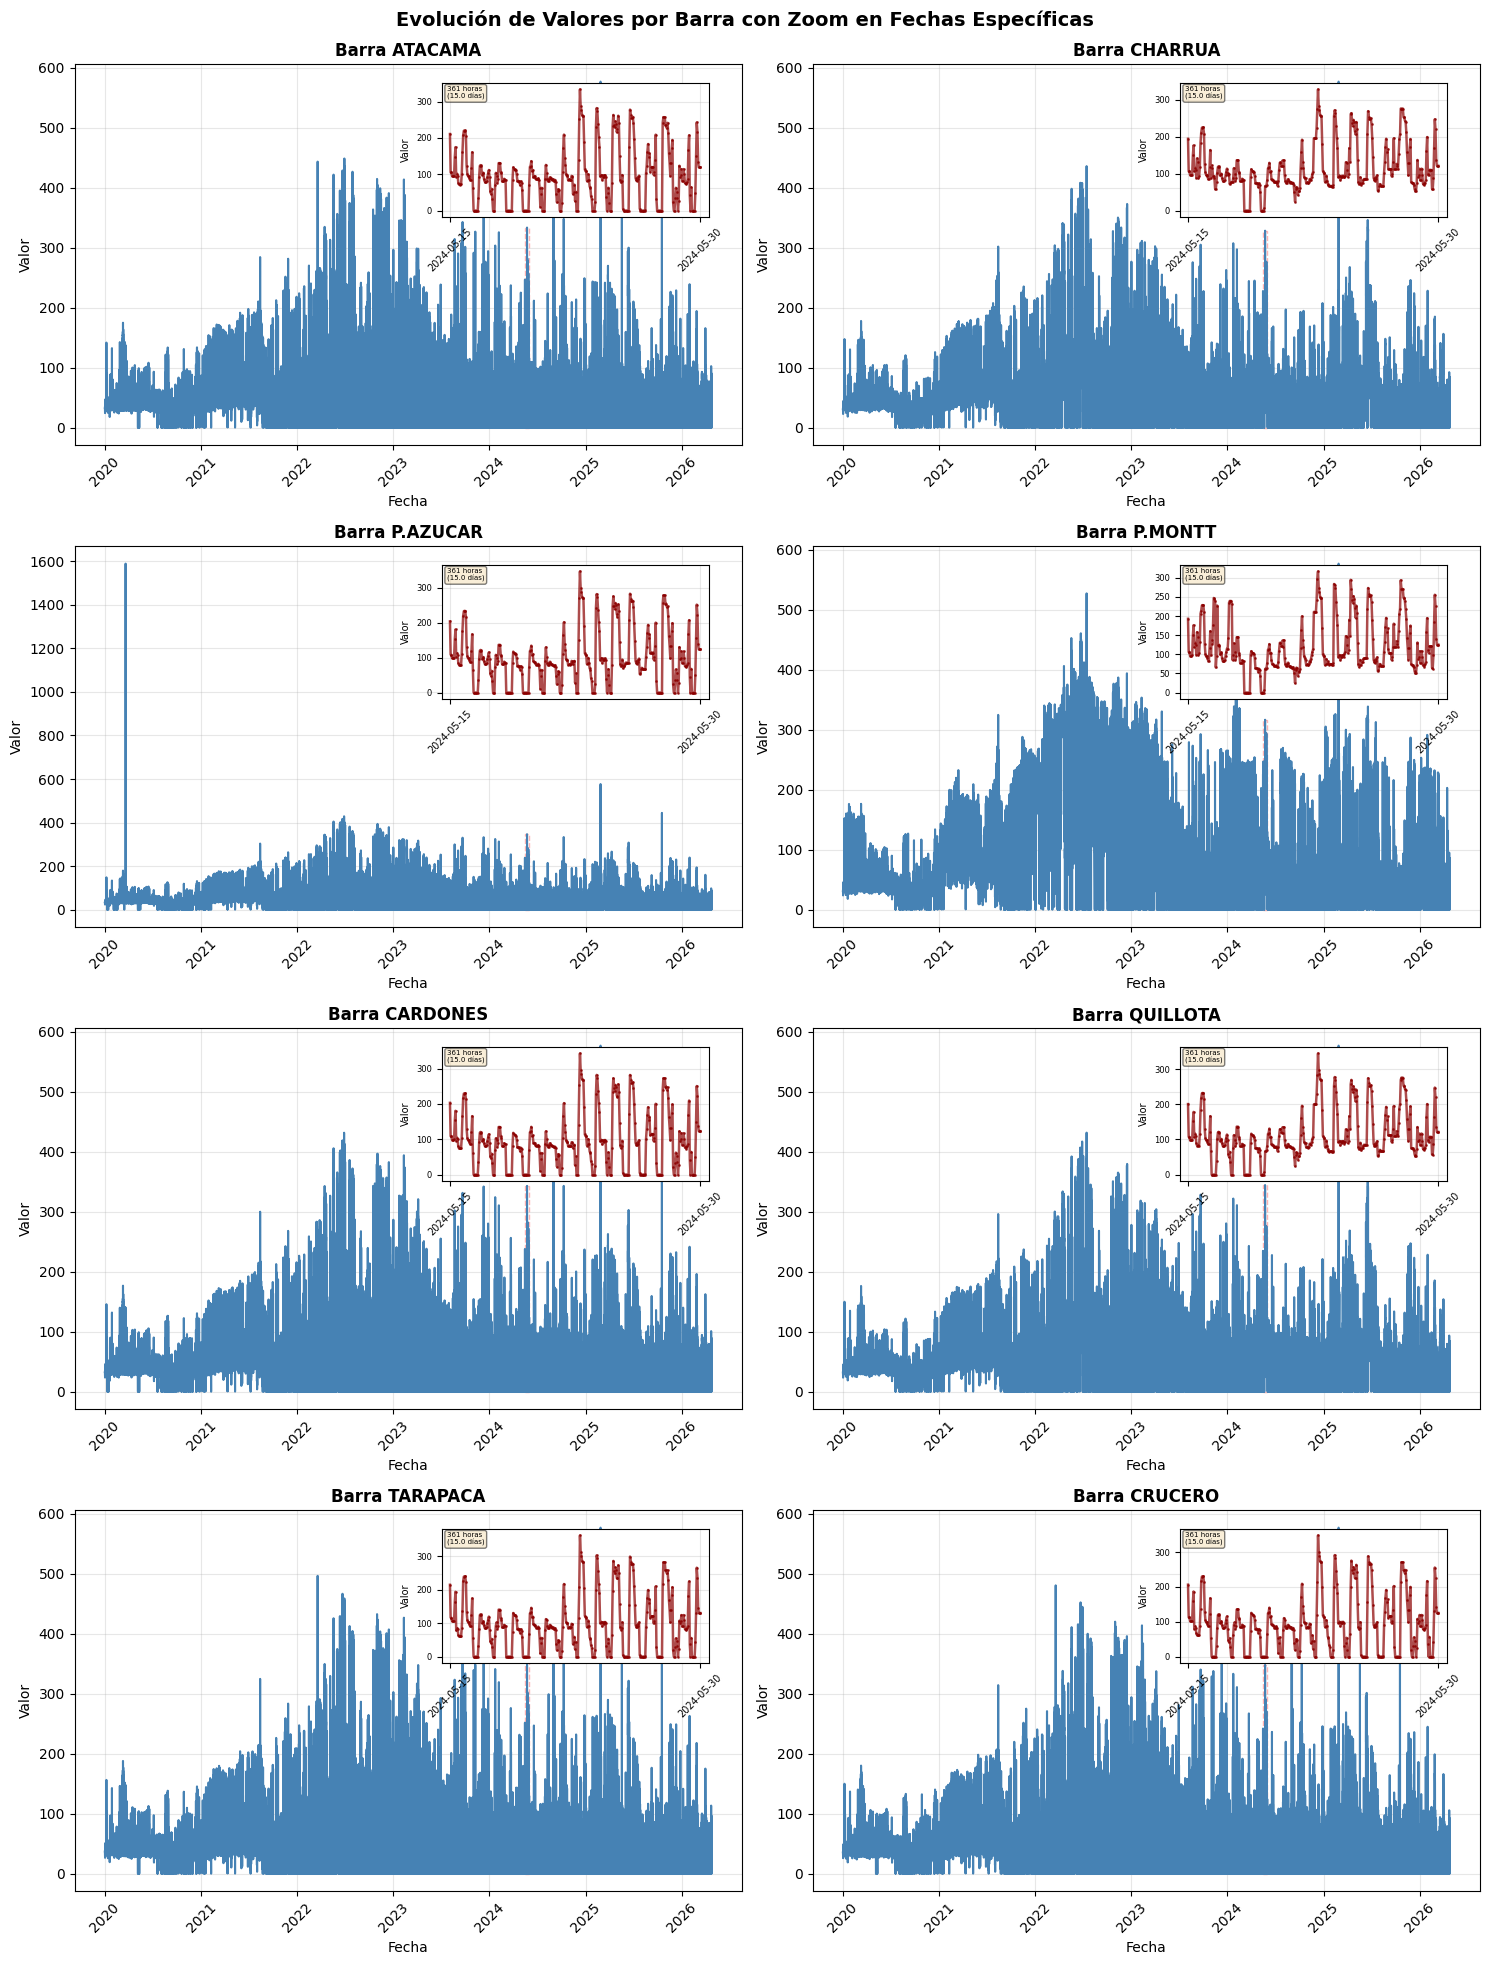
\includegraphics[width=0.9\linewidth]{imagenes/Posibles img/Serie Barras.png}
    \caption{Evolución del costo marginal horario para las ocho barras del SEN, período 2020--2026. Zoom en el período del 15/05/2024 - 30/05/2024}
    \label{fig:series_barras}
\end{figure}

Las series exhiben tres características estructurales relevantes. En primer lugar, presentan estacionalidad múltiple visible sobre todo a escala diaria y semanal, con un ciclo diario marcado por la caída del costo marginal durante el bloque solar y el alza en horas de menor radiación. En segundo lugar, se observan spikes de alta magnitud asociados a eventos de escasez hídrica, fallas de generación o congestiones de transmisión. En tercer lugar, se aprecia una tendencia decreciente en el nivel base del costo marginal a partir de 2022 en las barras del norte, consistente con la incorporación masiva de capacidad solar en esa zona del sistema.

La Tabla \ref{tab:estadisticas} resume las estadísticas descriptivas de cada barra. La heterogeneidad entre barras es marcada. Puerto Montt presenta la media más alta con 100.11 USD/MWh y la mayor desviación estándar con 94.05 USD/MWh, muy superior al resto de las barras, lo que refleja la influencia de la generación hidroeléctrica y su mayor variabilidad estacional asociada a los ciclos de precipitaciones. Las barras del norte, en cambio, presentan medias más bajas y medianas en el rango de \$54 a \$57 USD/MWh, coherente con la abundante generación solar que presiona el costo marginal hacia abajo durante el bloque diurno. El mínimo de 0.0 USD/MWh es común a todas las barras y corresponde a episodios de sobreoferta renovable donde el costo marginal colapsa. El caso más notable es la barra Pan de Azúcar, que registra un máximo de 1588.95 USD/MWh, considerablemente superior al máximo de 576.82 USD/MWh compartido por las demás barras, lo que refleja un evento extremo de congestión o escasez ocurrido cerca del año 2020, visible en la Figura \ref{fig:series_barras}. Este spike de magnitud excepcional constituye precisamente el tipo de evento que motiva el uso de DyT en la arquitectura TFT, por su capacidad de comprimir activaciones extremas de manera más robusta que LayerNorm, como se argumentó en la Sección 2.4.5.

\begin{table}[htbp]
    \centering
    \begin{tabular}{lrrrrr}
        \toprule
        Barra & Media & Desv. Est. & Mínimo & Mediana & Máximo \\
        \midrule
        Atacama       & 62.30  & 60.20 & 0.0 & 55.14 & 576.82   \\
        Cardones      & 62.37  & 59.75 & 0.0 & 55.01 & 576.82   \\
        Charrúa       & 66.21  & 58.87 & 0.0 & 57.35 & 576.82   \\
        Crucero       & 63.23  & 61.79 & 0.0 & 54.36 & 576.82   \\
        Pan de Azúcar & 63.26  & 60.32 & 0.0 & 56.40 & 1588.95 \\
        Puerto Montt  & 100.11 & 94.05 & 0.0 & 67.14 & 576.82   \\
        Quillota      & 66.74  & 58.79 & 0.0 & 59.09 & 576.82   \\
        Tarapacá      & 65.28  & 64.08 & 0.0 & 56.03 & 576.82   \\
        \bottomrule
    \end{tabular}
    \caption{Estadísticas descriptivas del costo marginal horario para las ocho barras del SEN, período 2020--2026.}
    \label{tab:estadisticas}
\end{table}

\subsection{Análisis de estacionariedad}

Para caracterizar formalmente las propiedades estadísticas de cada serie se aplican conjuntamente las pruebas ADF y KPSS descritas en la Sección 2.1.1. Los resultados se presentan en la Tabla \ref{tab:estacionariedad}.

\begin{table}[htbp]
    \centering
    \begin{tabular}{lcccc}
        \toprule
        Barra & Est. ADF & $p$-valor ADF & Est. KPSS & $p$-valor KPSS \\
        \midrule
        Atacama       & $-$13.2000 & $<0.001$ & 8.1252 & $<0.01$ \\
        Cardones      & $-$12.4464 & $<0.001$ & 8.1567 & $<0.01$ \\
        Charrúa       & $-$12.7728 & $<0.001$ & 8.4554 & $<0.01$ \\
        Crucero       & $-$12.6482 & $<0.001$ & 4.5352 & $<0.01$ \\
        Pan de Azúcar & $-$12.6063 & $<0.001$ & 7.2476 & $<0.01$ \\
        Puerto Montt  & $-$11.6217 & $<0.001$ & 4.8858 & $<0.01$ \\
        Quillota      & $-$12.7277 & $<0.001$ & 4.5890 & $<0.01$ \\
        Tarapacá      & $-$12.8396 & $<0.001$ & 8.2951 & $<0.01$ \\
        \bottomrule
    \end{tabular}
    \caption{Resultados de las pruebas de estacionariedad ADF y KPSS para las ocho barras.}
    \label{tab:estacionariedad}
\end{table}

El patrón es consistente en todas las barras: la prueba ADF rechaza la hipótesis nula de raíz unitaria con $p < 0.001$, evidencia de que las series no son paseos aleatorios puros y exhiben reversión a la media en el largo plazo. La prueba KPSS, en cambio, rechaza su hipótesis nula de estacionariedad en sentido débil con $p < 0.01$ (reportado en su valor límite inferior, dado que los estadísticos superan ampliamente los umbrales críticos de la librería). Esta combinación --rechazo simultáneo de ambas hipótesis nulas-- no es contradictoria, sino un patrón conocido en presencia de quiebres estructurales: el estadístico KPSS asume una serie que fluctúa en torno a un nivel (o tendencia) determinístico fijo, y tiende a rechazar la estacionariedad incluso cuando no existe una raíz unitaria genuina si ese nivel se desplaza gradualmente en el tiempo, como es esperable dada la incorporación continua de capacidad renovable al SEN durante el período de datos (Sección 3.1). En conjunto, ambas pruebas son consistentes con series que revierten a la media en el largo plazo (sin raíz unitaria, según ADF) pero cuyo nivel base no es fijo sino que se desplaza gradualmente (lo que basta para que KPSS rechace la estacionariedad, sin que esto implique nada directamente sobre la varianza de la serie). Esta caracterización, centrada en el nivel de la serie más que en su varianza, justifica específicamente el uso de Prophet con detección automática de puntos de quiebre, que modela explícitamente esos desplazamientos graduales de nivel. La heterocedasticidad asociada a los \textit{spikes} de alta magnitud, visible en las estadísticas descriptivas de la Tabla \ref{tab:estadisticas}, es una propiedad adicional de la serie --no algo que ADF o KPSS, ambas centradas en la dinámica del nivel, permitan concluir por sí solas-- y es la que motiva, de forma independiente, la estandarización z-score como transformación de preprocesamiento.

\section{Preprocesamiento}

El preprocesamiento de los datos se realiza en dos etapas diferenciadas según el modelo destino, dado que Prophet y el TFT tienen requisitos distintos respecto a la escala de los datos.

\subsection{Limpieza y tratamiento de valores atípicos}

En primer lugar se verifica la integridad de la serie temporal. Los datos del CEN no presentan valores faltantes en el período estudiado; no obstante, el pipeline contempla interpolación lineal como mecanismo de contingencia ante eventuales ausencias puntuales, preservando así la continuidad temporal de la serie sin introducir sesgos hacia valores futuros.

En segundo lugar se tratan los outliers. Dado que las series de costo marginal presentan spikes de alta magnitud asociados a eventos excepcionales, se aplica un umbral de 4 desviaciones estándar calculadas sobre el conjunto de entrenamiento: las observaciones que superan $\hat{\mu} + 4\hat{\sigma}$ se reemplazan mediante interpolación lineal entre los valores adyacentes. Este umbral es suficientemente amplio para preservar los spikes estructurales del mercado, como los episodios de escasez hídrica o congestión de transmisión, que son parte de la dinámica real del sistema y deben ser aprendidos por el modelo, mientras elimina únicamente los valores de magnitud excepcional que podrían distorsionar el entrenamiento, como el spike de 1.588,95 USD/MWh registrado en la barra Pan de Azúcar. El umbral se estima exclusivamente sobre el conjunto de entrenamiento y se aplica sin reestimación al resto de los conjuntos, evitando data leakage.

\subsection{División temporal de los datos}

Los datos se dividen en tres conjuntos cronológicamente ordenados, respetando estrictamente la causalidad temporal: ningún conjunto contiene observaciones posteriores a las del conjunto siguiente. La división adoptada es 70\% entrenamiento, 15\% validación y 15\% test, que corresponde a los siguientes períodos:

\begin{table}[htbp]
    \centering
    \begin{tabular}{llll}
        \toprule
        Conjunto & Inicio & Término & Proporción \\
        \midrule
        Entrenamiento & 2020-01-01 01:00 & 2024-06-01 12:00 & 70\% \\
        Validación    & 2024-06-01 13:00 & 2025-05-13 06:00 & 15\% \\
        Test          & 2025-05-13 07:00 & 2026-04-24 00:00 & 15\% \\
        \bottomrule
    \end{tabular}
    \caption{División temporal de los datos por conjunto.}
    \label{tab:division}
\end{table}

El conjunto de entrenamiento cubre el período 2020--2024, que incluye la transición energética acelerada y los episodios de sobreoferta solar de los primeros años. El conjunto de validación, comprendido entre junio de 2024 y mayo de 2025, se utiliza para la optimización de hiperparámetros de Prophet, la selección del mejor ensamble en el Stacking Optimization y el ajuste de los pesos de combinación. El conjunto de prueba, de mayo de 2025 a abril de 2026, se reserva exclusivamente para la evaluación final del modelo y la construcción de los intervalos de Conformal Prediction, y no es accedido en ninguna etapa del entrenamiento ni de la selección de modelos.

\subsection{Normalización}

La normalización se aplica de manera diferenciada según el modelo. Prophet opera directamente sobre los valores originales del costo marginal en USD/MWh, dado que su formulación aditiva es interpretable en la escala original y sus componentes de tendencia y estacionalidad tienen significado físico directo en esa escala.

Para el TFT, en cambio, se aplica estandarización z-score independientemente para cada barra:

\begin{equation}
    \tilde{y}_t^{(b)} = \frac{y_t^{(b)} - \hat{\mu}^{(b)}}{\hat{\sigma}^{(b)}}
\end{equation}

donde $\hat{\mu}^{(b)}$ y $\hat{\sigma}^{(b)}$ son la media y desviación estándar estimadas exclusivamente sobre el conjunto de entrenamiento de la barra $b$. La normalización independiente por barra es necesaria porque las series presentan niveles y variabilidades distintas, como se evidencia en la Tabla \ref{tab:estadisticas}, donde Puerto Montt tiene una media de 100.11 USD/MWh frente a las barras del norte con medias en torno a 62--66 USD/MWh. Aplicar una normalización conjunta introduciría un sesgo sistemático en las barras con niveles más extremos. Los parámetros $\hat{\mu}^{(b)}$ y $\hat{\sigma}^{(b)}$ se aplican sin reestimación a los conjuntos de validación y prueba, preservando la integridad de la evaluación fuera de muestra.

\section{Modelo Prophet}

\subsection{Configuración y optimización de hiperparámetros}

Prophet se entrena sin transformación previa, sobre los valores originales del costo marginal en USD/MWh (Sección 3.2.3). Se incorporan los feriados nacionales del calendario chileno como variable exógena mediante el argumento \texttt{holidays}, capturando el efecto sistemático de los días festivos sobre el despacho del SEN descrito en la Sección 2.2.3. Las estacionalidades diaria, semanal y anual se activan explícitamente. El tipo de tendencia se fija como lineal por tramos (\texttt{growth='linear'}), adecuado para series de precios que no tienen una capacidad de saturación definida. Además, esta decisión de diseño está motivada por las dificultades prácticas en la implementación del modo multiplicativo: Prophet requiere la especificación explícita de valores de techo y piso para ese modo, parámetros que no tienen una interpretación directa en series de costos marginales sin capacidad de saturación definida, y el entrenamiento con modo multiplicativo presentó tiempos de cómputo significativamente mayores sin mejoras observables en validación preliminar. La búsqueda se realiza mediante grid search minimizando el MAE sobre el conjunto de validación, preservando la causalidad temporal.

Los hiperparámetros optimizados son \texttt{changepoint\_prior\_scale} (CPS), que controla la flexibilidad de la tendencia lineal por tramos, y \texttt{seasonality\_prior\_scale} (SPS), que controla la flexibilidad de las componentes estacionales, ambos descritos en la Sección 2.2. La Tabla~\ref{tab:prophet_params} presenta los hiperparámetros óptimos encontrados para cada barra.

\begin{table}[htbp]
    \centering
    \begin{tabular}{lccc}
        \toprule
        Barra & CPS & SPS & MAE val. \\
        \midrule
        Atacama       & 0.02 & 0.2   & 21.54 \\
        Cardones      & 0.05 & 5.0   & 21.89 \\
        Charrúa       & 0.02 & 0.01  & 24.30 \\
        Crucero       & 0.05 & 0.007 & 22.25 \\
        Pan de Azúcar & 0.05 & 0.007 & 22.66 \\
        Puerto Montt  & 0.05 & 0.01  & 46.01 \\
        Quillota      & 0.02 & 1.0   & 23.77 \\
        Tarapacá      & 0.05 & 0.01  & 23.09 \\
        \bottomrule
    \end{tabular}
    \vspace{0.2cm}
    \caption{Hiperparámetros óptimos de Prophet por barra. MAE en conjunto de validación (USD/MWh).}
    \label{tab:prophet_params}
\end{table}

Dos patrones emergen de los resultados. Primero, los valores de CPS son bajos en todas las barras (0.02--0.05), indicando que Prophet prefiere tendencias suaves con pocos cambios abruptos, consistente con los cambios estructurales graduales del mercado descritos en la Sección 3.1. Segundo, los valores de SPS son notablemente bajos en la mayoría de las barras (0.007--0.01), lo que indica que con datos horarios Prophet prefiere estacionalidades rígidas, posiblemente porque la alta densidad temporal de las observaciones ya provee suficiente información para estimar los patrones estacionales sin necesidad de flexibilidad adicional. Las excepciones son Cardones (SPS=5.0) y Quillota (SPS=1.0), cuyas estacionalidades requieren mayor adaptabilidad, y Atacama (SPS=0.2), que ocupa una posición intermedia.

\subsection{Componentes de tendencia y estacionalidad anual}

La Figura \ref{fig:prophet_trend_yearly} presenta las componentes de tendencia y de estacionalidad anual estimadas por Prophet para las ocho barras, período 2020--2026.

\begin{figure}[htbp]
    \centering
    \begin{minipage}[t]{0.48\textwidth}
        \centering
        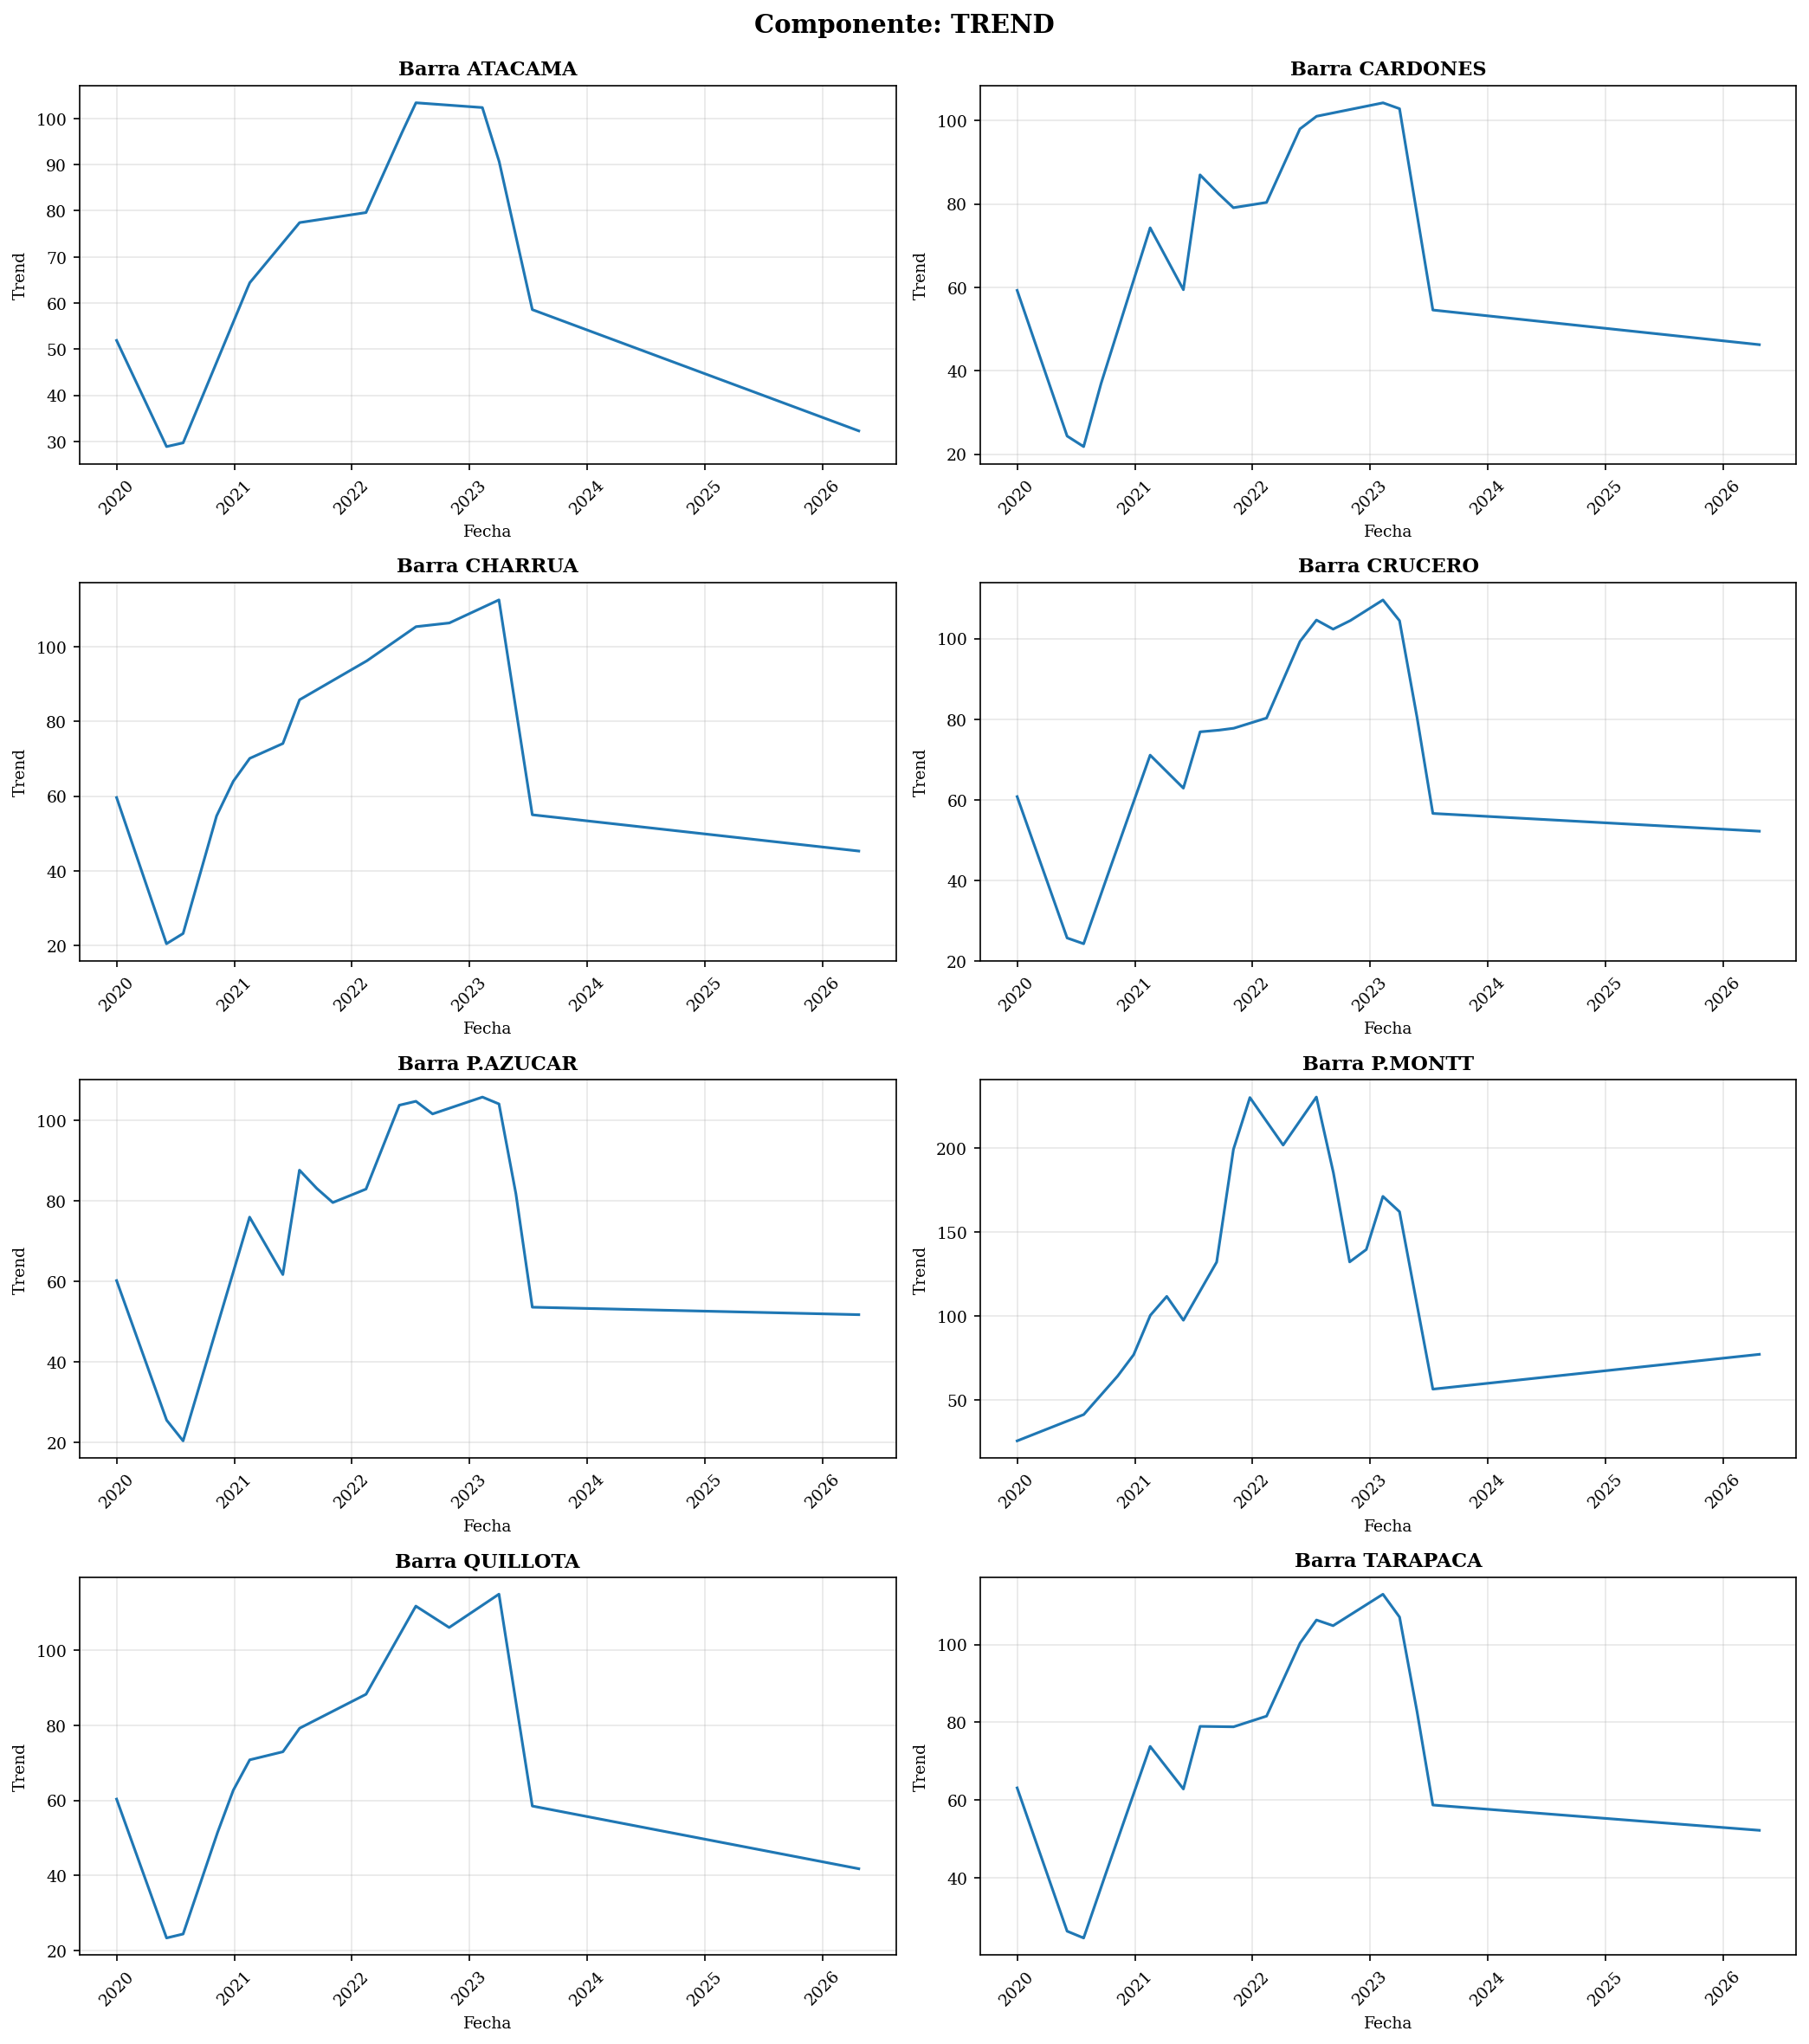
\includegraphics[width=\textwidth]{imagenes/Posibles img/Componente Trend.png}
        \caption*{Tendencia}
    \end{minipage}
    \hfill
    \begin{minipage}[t]{0.48\textwidth}
        \centering
        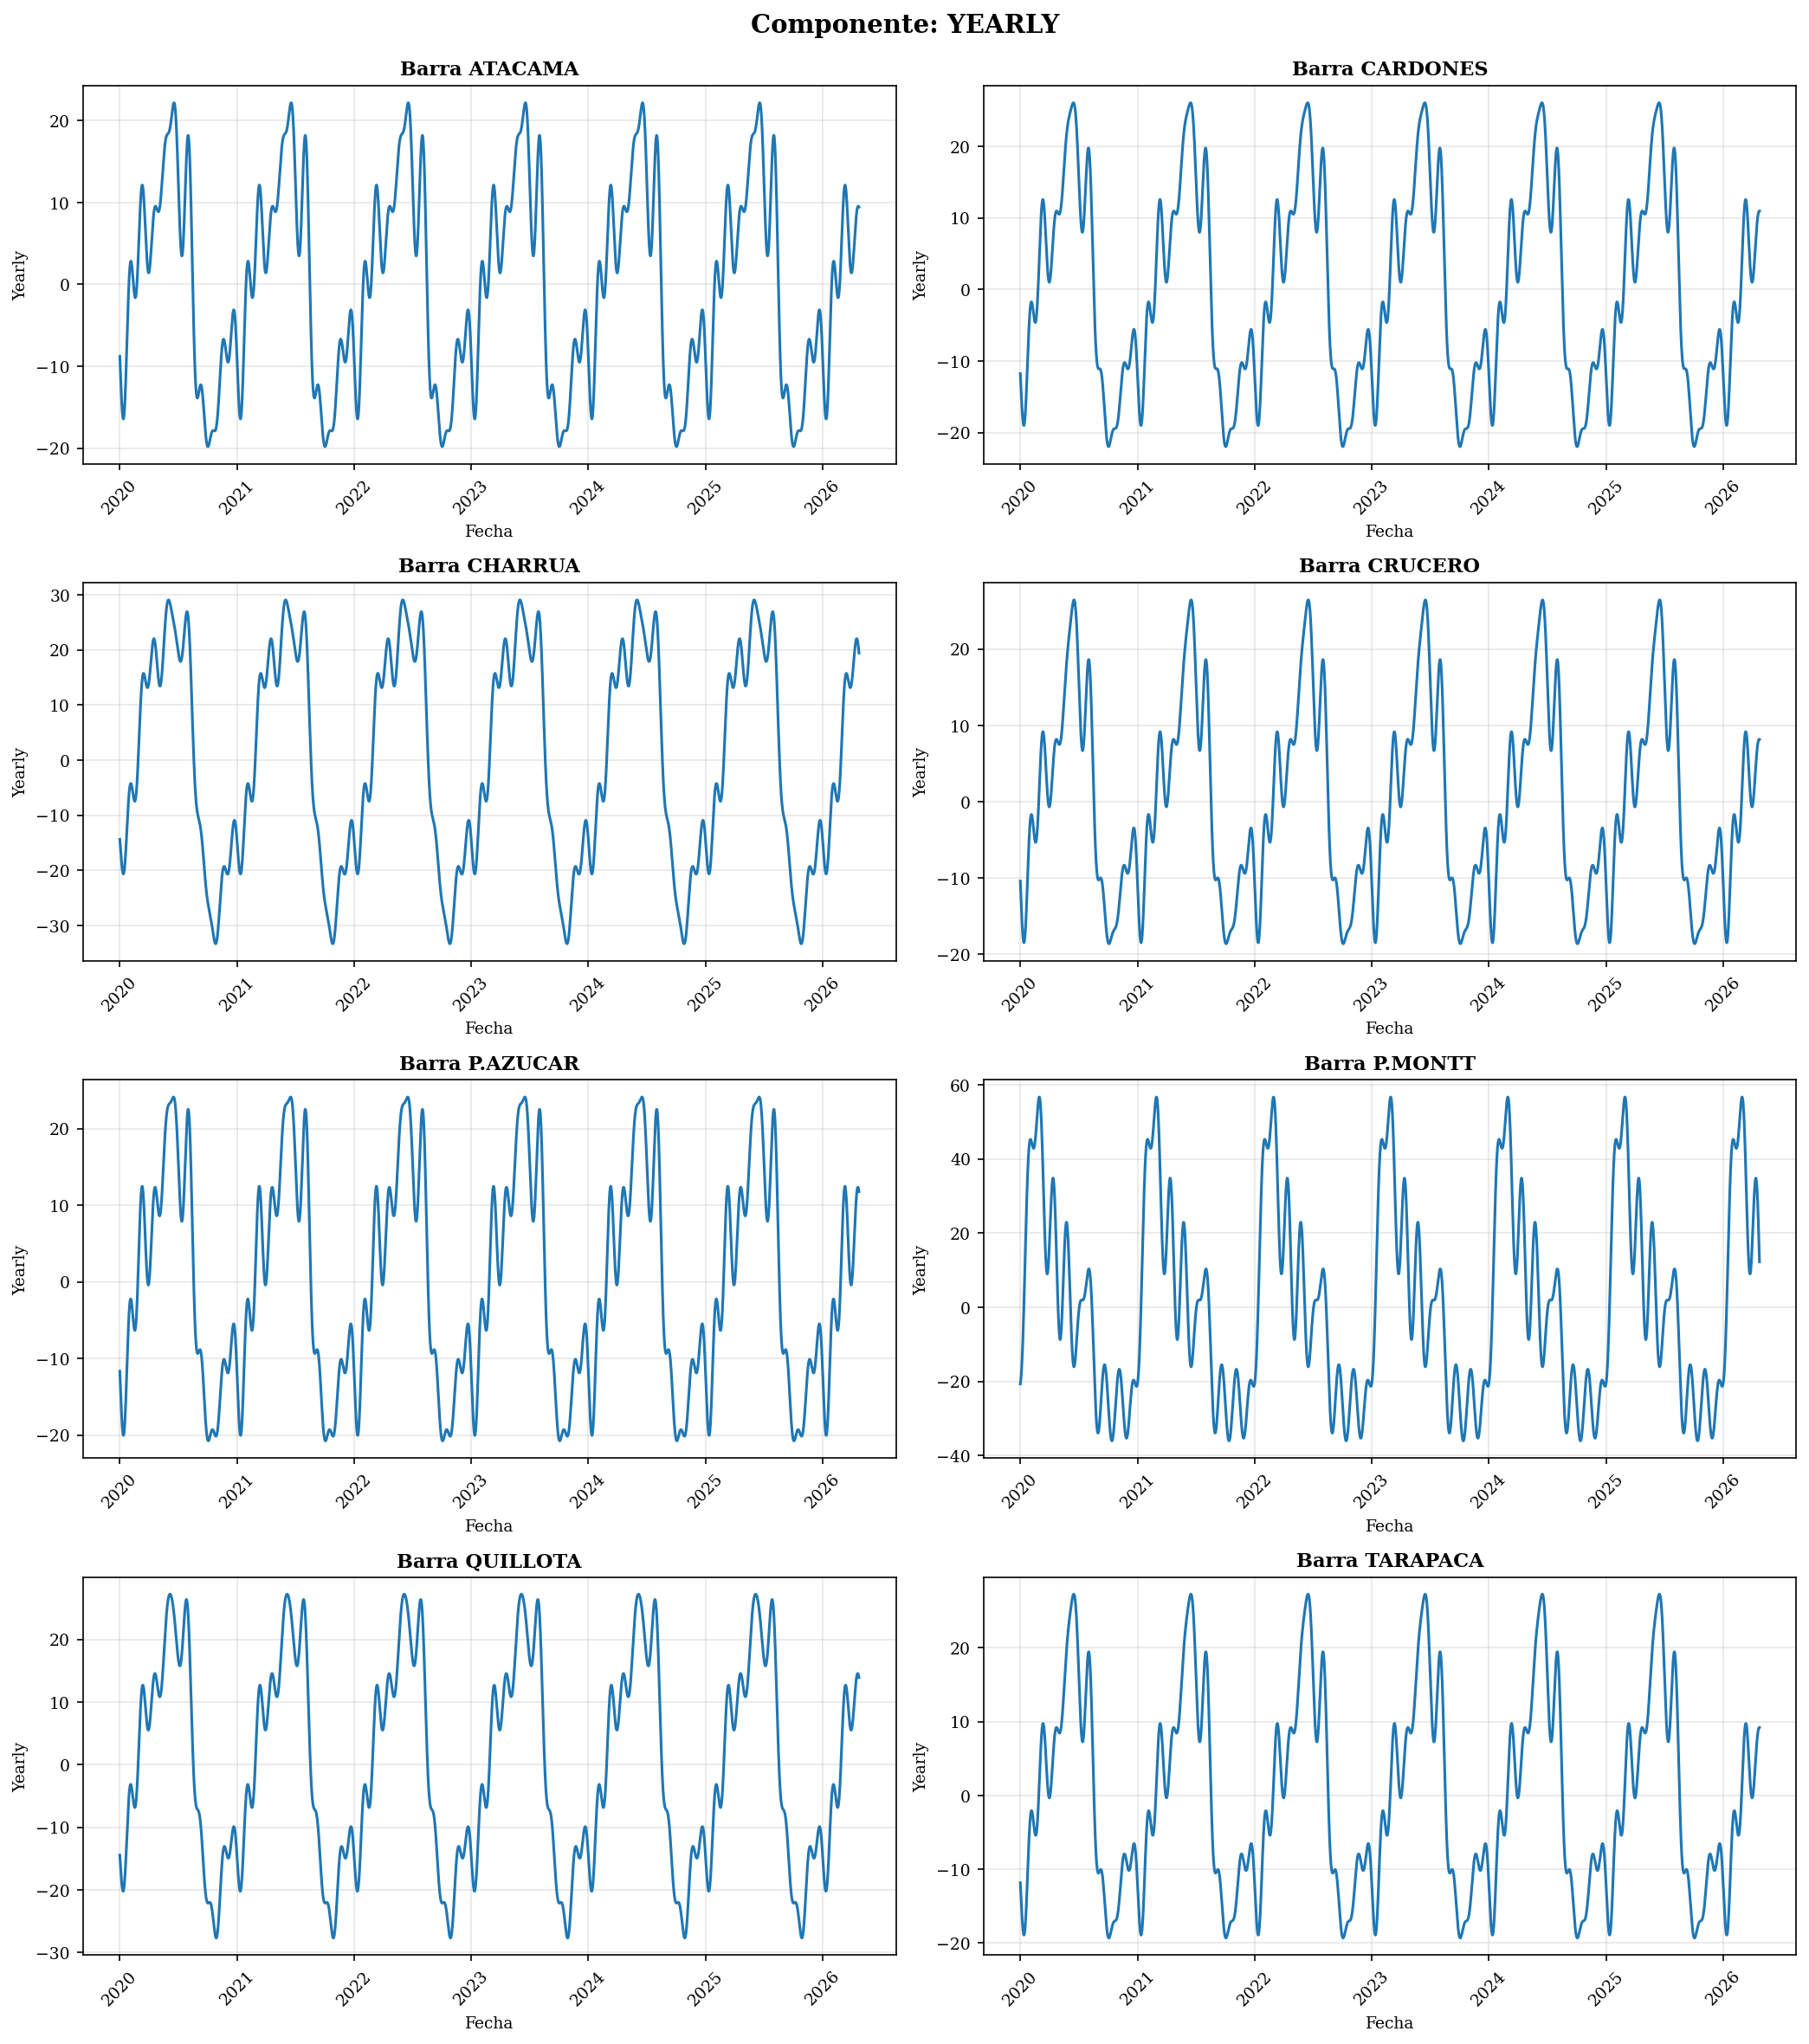
\includegraphics[width=\textwidth]{imagenes/Posibles img/Componente Yearly.png}
        \caption*{Estacionalidad anual}
    \end{minipage}
    \caption{Componentes de tendencia y de estacionalidad anual estimadas por Prophet para las ocho barras del SEN, período 2020--2026.}
    \label{fig:prophet_trend_yearly}
\end{figure}

La tendencia revela un patrón común a todas las barras: una fase de alza sostenida entre 2020 y 2022--2023, consistente con la recuperación post-pandemia y la alta demanda de ese período, seguida de una caída pronunciada desde 2024 que refleja la incorporación masiva de capacidad solar y eólica. La componente anual, por su parte, muestra una amplitud moderada de $\pm$20--30 USD/MWh en las barras del norte, asociada al ciclo estacional de la radiación solar. Puerto Montt es la excepción en ambas componentes: una tendencia con niveles muy superiores (en torno a 200 USD/MWh en el peak de 2022--2023) y una caída más abrupta, y la mayor amplitud anual del grupo ($\pm$60 USD/MWh), consistentes con la dependencia de los ciclos hidrológicos de deshielo y precipitaciones que rigen la generación hidroeléctrica del sur.

\subsection{Predicciones a 48 horas}

La Figura \ref{fig:prophet_pred48} ilustra las predicciones de Prophet para un horizonte de 48 horas a partir del último instante del conjunto de prueba, mostrando el histórico reciente y la proyección para cada barra.

\begin{figure}[htbp]
    \centering
    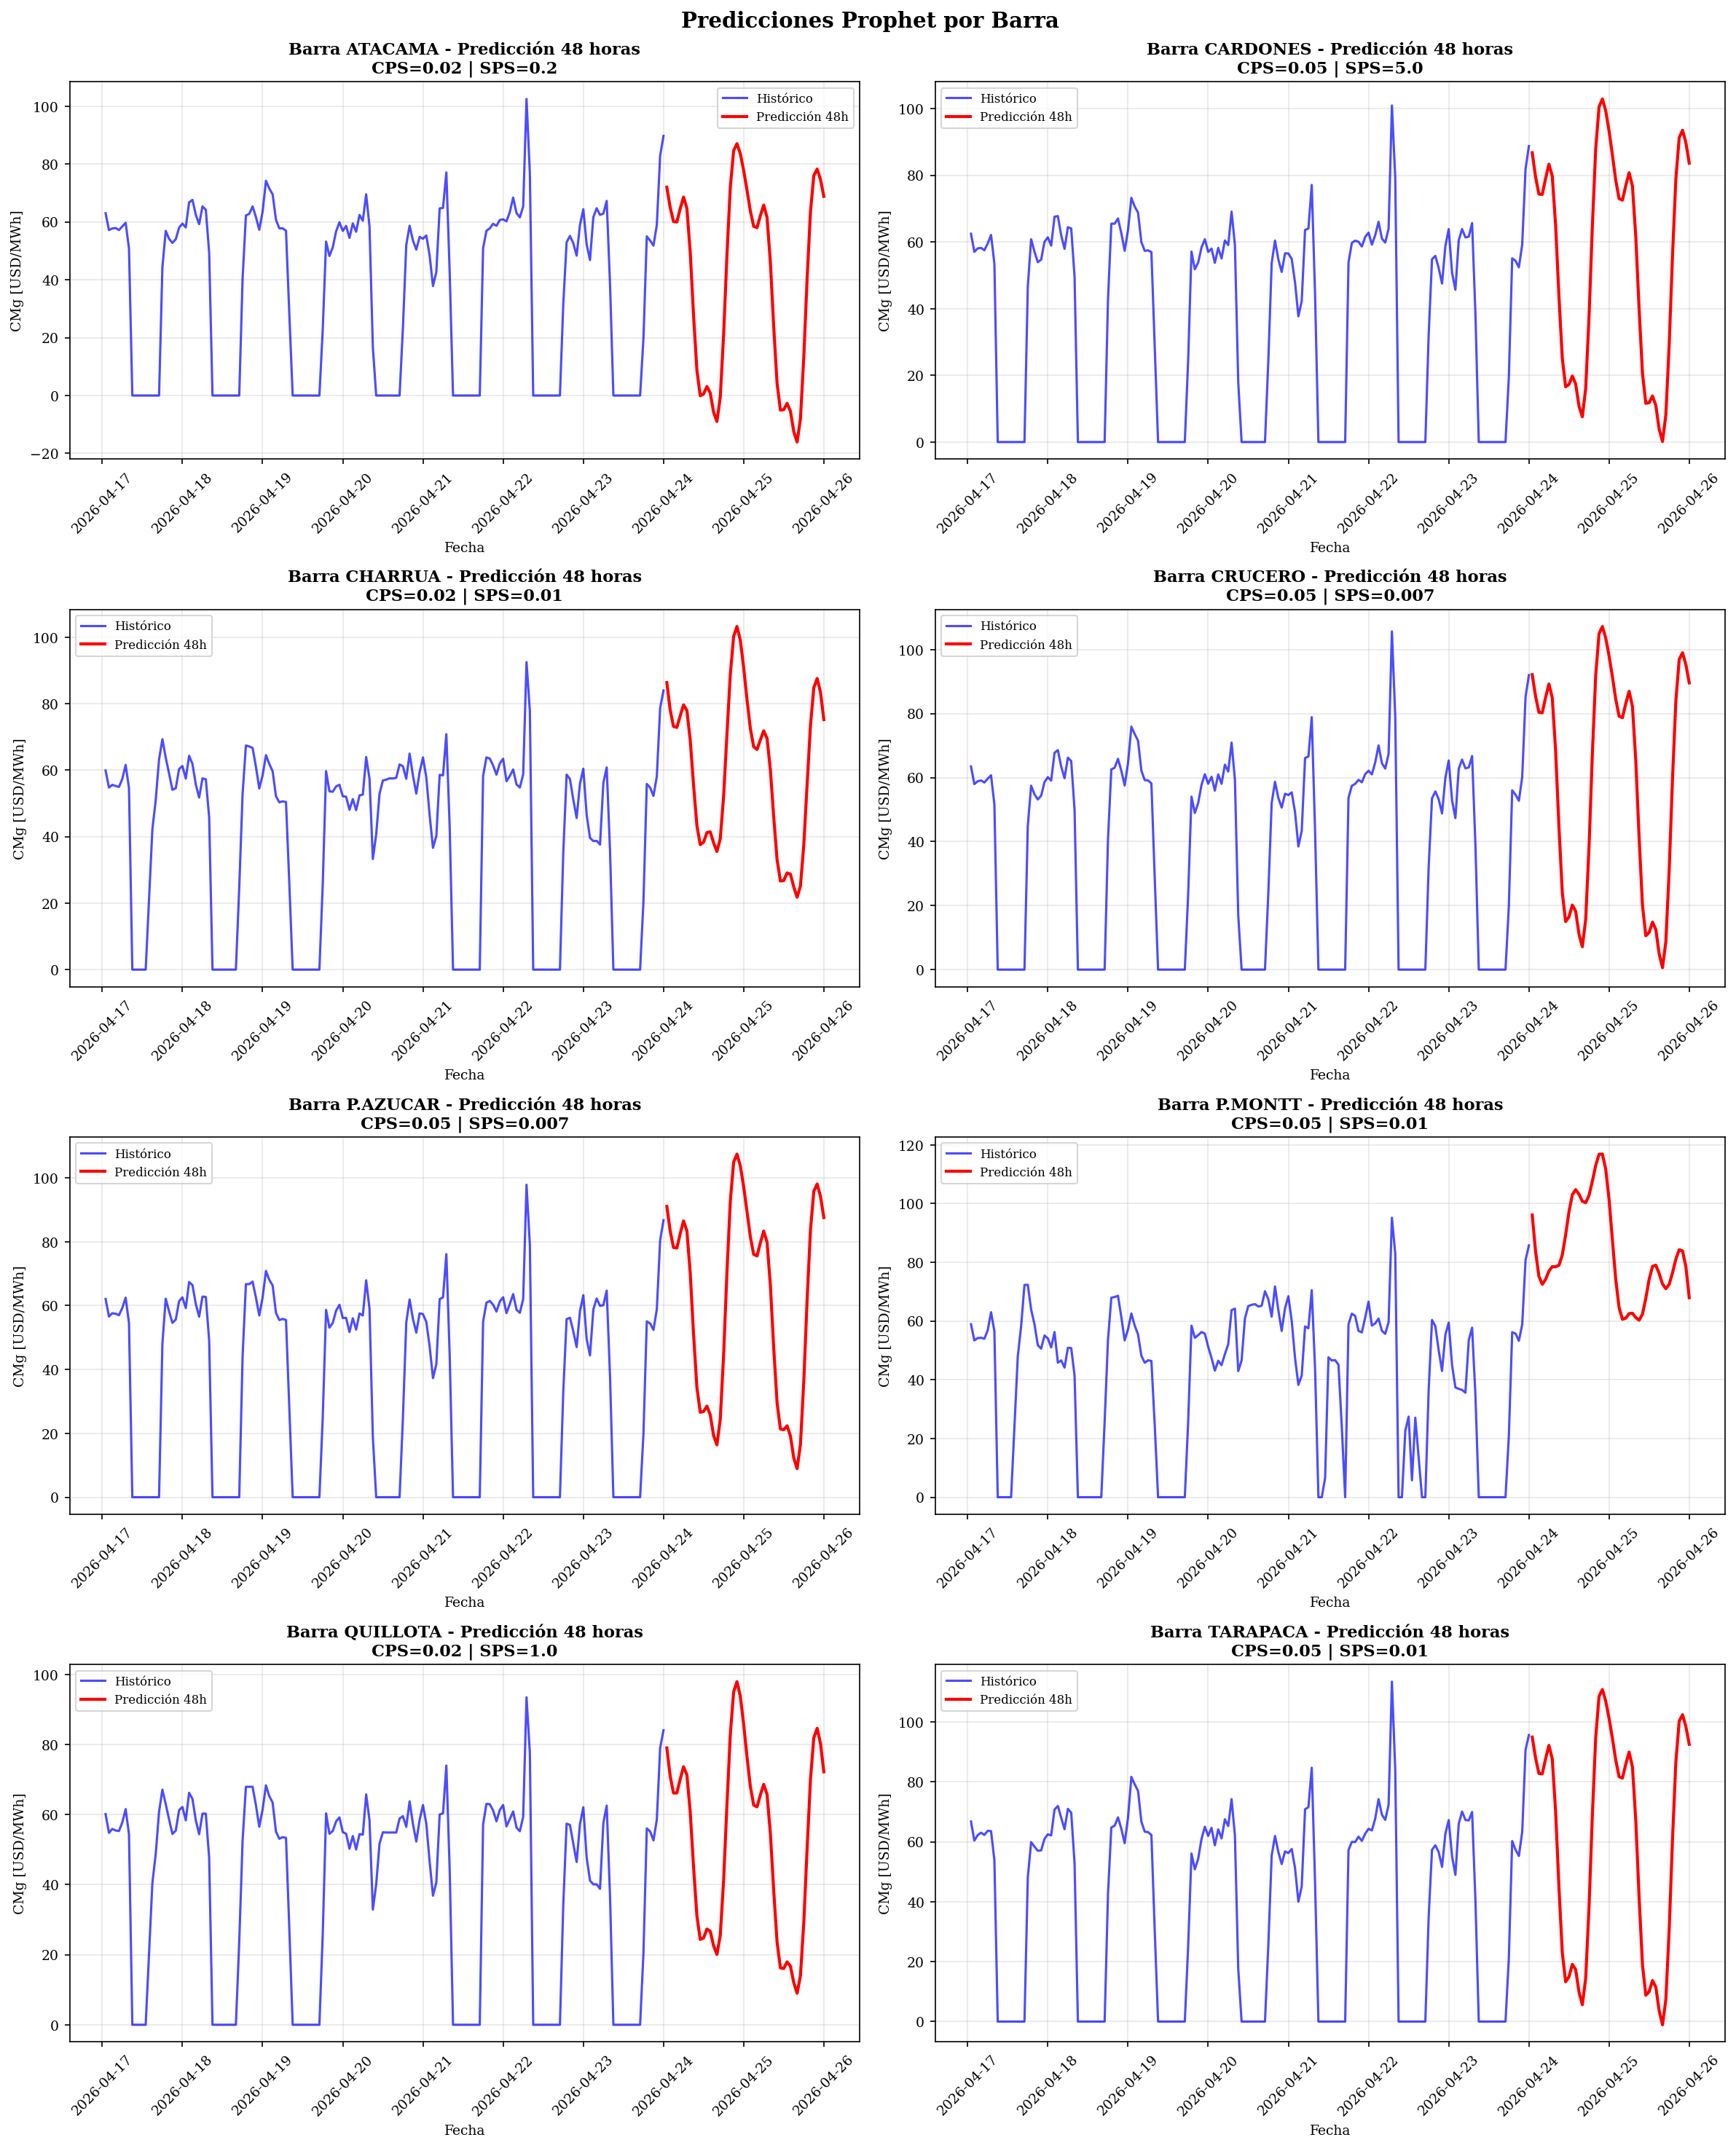
\includegraphics[width=0.95\textwidth]{imagenes/Posibles img/Predicciones por Barra.png}
    \caption{Predicciones de Prophet a 48 horas para las ocho barras del SEN, mostrando el histórico reciente (azul) y la proyección (rojo). Se aprecia el ciclo diario capturado por el modelo, con la caída característica durante el bloque solar y el alza en horas nocturnas.}
    \label{fig:prophet_pred48}
\end{figure}

Las predicciones a 48 horas confirman que Prophet captura correctamente la estructura del ciclo diario, reproduciendo la caída característica durante el bloque solar y el alza en horas de menor generación renovable. Sin embargo, se observa que en algunas barras la predicción alcanza valores negativos, lo que constituye una limitación física del modelo: el costo marginal no puede ser negativo en el SEN, pero Prophet, al ser un modelo de descomposición aditiva sin restricciones de dominio, puede extrapolar fuera del rango físicamente válido cuando la componente estacional supera a la tendencia. Esta limitación es inherente a la formulación de Prophet y refuerza la necesidad del TFT como componente complementario, cuya arquitectura de red neuronal le permite aprender implícitamente los límites del rango observado. Las predicciones de Prophet reportadas en el Capítulo 4 se truncan en 0 USD/MWh para evitar que esta limitación degrade artificialmente sus métricas de evaluación (Sección \ref{sec:modelo_prophet}); el residuo que consume $\text{TFT}_\text{LN}$ en la rama P+C, en cambio, se calcula sobre la predicción sin truncar, dado que truncarlo exigiría reentrenar el modelo de residuos sobre el nuevo objetivo.

\section{Temporal Fusion Transformer}

\subsection{Construcción de features y dataloaders}

El TFT recibe los datos estandarizados, según la transformación descrita en la Sección 3.2, junto con un conjunto de features organizadas en tres grupos según la taxonomía del TFT descrita en la Sección 2.3.4: covariables estáticas, covariables temporales conocidas (\texttt{known\_reals}) y covariables temporales desconocidas (\texttt{unknown\_reals}).

Se comparan dos estrategias de construcción de \texttt{known\_reals}, que constituyen las dos ramas metodológicas centrales evaluadas en este trabajo:

\begin{itemize}
    \item \textbf{Prophet + Clima (P+C):} las \texttt{known\_reals} corresponden a las cuatro componentes descompuestas por Prophet, tendencia (\texttt{trend}), estacionalidad anual (\texttt{yearly}), semanal (\texttt{weekly}) y diaria (\texttt{daily}), más un indicador binario de feriado nacional (\texttt{is\_holiday}). Es la estrategia originalmente adoptada en el diseño del modelo híbrido, dado que motiva directamente el esquema de ensamblaje Prophet-TFT descrito en la Sección 3.5.
    \item \textbf{Sol + Clima (S+C):} las \texttt{known\_reals} se reemplazan por tres variables de posición solar calculadas directamente mediante la librería \texttt{pvlib}: un indicador binario de horario de verano (\texttt{es\_horario\_verano}), el ángulo de elevación solar (\texttt{elevacion\_solar}) y su coseno (\texttt{cos\_elevacion}). El ángulo de elevación se obtiene mediante la función \texttt{get\_solarposition} del módulo \texttt{solarposition} de \texttt{pvlib}, aplicada sobre la marca temporal en UTC, calculada a partir de la hora local chilena considerando explícitamente los cambios de huso horario de verano/invierno, que en Chile no siguen una regla fija de calendario sino fechas específicas determinadas por decreto cada año; las coordenadas geográficas usadas para cada barra se detallan más adelante en esta subsección, junto con las variables climáticas.
\end{itemize}

La motivación de la rama S+C es evitar la dependencia de un modelo de descomposición intermedio para representar el ciclo diario y anual del costo marginal: la elevación solar es una variable física directamente observable que captura ambos ciclos de forma más directa que las componentes estimadas por Prophet, sin requerir un proceso de ajuste propio ni estar sujeta a los supuestos de la descomposición aditiva. Ambas ramas se evalúan de forma independiente (Prophet cuando corresponde, TFT de precios y de residuos, Stacking Optimization, TFT con DyT y Conformal Prediction) y se comparan empíricamente en el Capítulo 4.

Las \textit{covariables estáticas} incluyen, en ambas ramas, el identificador de barra (\texttt{serie\_id}), que permite al modelo aprender dinámicas temporales distintas para cada nodo del sistema sin necesidad de entrenar instancias separadas, tal como se describió en la Sección 2.3.4.

Las \textit{covariables temporales desconocidas} (\texttt{unknown\_reals}) son las mismas en ambas ramas. Para el TFT de precios corresponden a la serie estandarizada (\texttt{y\_real}) más las cinco variables climáticas horarias. Para el TFT de residuos, utilizado únicamente en la rama P+C dado que la rama S+C no calcula residuos de Prophet, corresponden al residuo estandarizado (\texttt{residuo}) más las mismas cinco variables climáticas. Deliberadamente no se incluyen lags manuales (por ejemplo, de 1, 24 o 168 horas) ni estadísticos móviles (medias o desviaciones estándar sobre ventanas de 24 o 168 horas): estas dependencias de corto y largo plazo se delegan íntegramente al mecanismo de atención y a las capas LSTM del encoder de 168 horas descrito a continuación, evitando representar explícitamente una estructura temporal que el modelo ya captura internamente.

Las variables climáticas corresponden a temperatura a 2 metros (\texttt{temperatura}), humedad relativa (\texttt{humedad}), velocidad del viento a 10 metros (\texttt{velocidad\_viento}), precipitación (\texttt{precipitacion}) y nubosidad (\texttt{nubosidad}), obtenidas con resolución horaria desde la API de archivo de Open-Meteo (\texttt{archive-api.open-meteo.com}), que provee datos de reanálisis ERA5 del Centro Europeo de Predicción Meteorológica a Medio Plazo (ECMWF). Los datos se obtienen para las coordenadas geográficas de la ciudad más representativa de cada barra: Iquique para Tarapacá, Antofagasta para Crucero, Copiapó para Cardones, Vallenar para Atacama, La Serena para Pan de Azúcar, Valparaíso para Quillota, Concepción para Charrúa y Puerto Montt para la barra homónima.

Cabe declarar una limitación de viabilidad operacional de esta fuente de datos, independiente de la validez causal del esquema \texttt{unknown\_reals}: ERA5 es un producto de reanálisis, no una observación en tiempo real, y se publica con un rezago del orden de días respecto de la fecha a la que corresponde. Esto significa que, aunque el modelo nunca recibe clima de horas futuras a la que predice --las cinco variables entran como \texttt{unknown\_reals}, solo disponibles para el encoder, nunca para el paso del decoder-- ni siquiera el clima de las horas más recientes de la propia ventana de encoder estaría disponible en operación real al momento de generar una predicción, porque ERA5 para esos días recientes todavía no ha sido publicado. El pipeline evaluado en este trabajo es, por lo tanto, causalmente correcto pero no directamente desplegable tal cual: una implementación operacional requeriría sustituir ERA5 por un producto de pronóstico meteorológico a corto plazo (por ejemplo, GFS o el pronóstico operacional de ECMWF) para las horas más recientes de la ventana de encoder, cuyo error de pronóstico degradaría en algún grado el desempeño reportado en el Capítulo 4. Evaluar esa degradación queda fuera del alcance de este trabajo.

La ventana de contexto se fija en $L = 168$ horas, equivalente a una semana completa, lo que permite al TFT acceder a un ciclo semanal completo de historia al realizar cada predicción. El horizonte de predicción es $h = 1$ hora, consistente con el objetivo de forecasting definido en la Sección 2.1.4. Para cada instante de predicción, el encoder mínimo se fija en $L/2 = 84$ horas para garantizar que todas las ventanas de entrenamiento tengan contexto suficiente. PyTorch Forecasting agrega automáticamente el índice de tiempo relativo (\texttt{add\_relative\_time\_idx}) y las escalas del target (\texttt{add\_target\_scales}) como features adicionales. Una ventana de contexto de dos semanas ($L = 336$ horas) y de 10 días ($L = 240$ horas) fue evaluada preliminarmente: el entrenamiento no fallaba de inmediato, pero colapsaba por falta de memoria hacia las épocas 10--15, y si bien hubiese sido posible reanudar el entrenamiento desde el último checkpoint guardado, el tiempo adicional requerido para completar las 100 épocas de esta forma no era viable dentro del presupuesto computacional del trabajo. Por lo tanto, $L = 168$ horas constituye el máximo viable bajo las restricciones computacionales del trabajo.

Los dataloaders se construyen de manera que el conjunto de validación incluye el período de entrenamiento más el de validación, y el conjunto de prueba incluye los tres períodos concatenados, preservando la continuidad del índice temporal (\texttt{time\_idx}) en todo momento. Se verifica explícitamente que el índice sea monótonamente creciente en cada conjunto para garantizar la causalidad temporal.

\subsection{Arquitectura y entrenamiento}

Los hiperparámetros del TFT se presentan en la Tabla \ref{tab:tft_config}. En la rama P+C se entrenan dos instancias del TFT con la misma configuración: una sobre la serie estandarizada de precios ($\text{TFT}_\text{LN}$ precios) y otra sobre los residuos de Prophet ($\text{TFT}_\text{LN}$ residuos); en la rama S+C se entrena únicamente la instancia de precios, dado que no existe un residuo de Prophet que modelar.

\begin{table}[htbp]
    \centering
    \begin{tabular}{ll}
        \toprule
        Hiperparámetro & Valor \\
        \midrule
        Learning rate inicial         & 0.001 \\
        Hidden size                   & 32 \\
        Attention heads               & 4 \\
        Dropout                       & 0.2 \\
        Hidden continuous size        & 8 \\
        Función de pérdida            & MAE \\
        Épocas máximas                & 100 \\
        Early stopping patience       & 15 épocas \\
        Reduce LR on plateau patience & 5 épocas \\
        Gradient clipping             & 0.1 \\
        Ventana de contexto $L$       & 168 horas \\
        Horizonte $h$                 & 1 hora \\
        \bottomrule
    \end{tabular}
    \caption{Hiperparámetros del TFT con LayerNorm.}
    \label{tab:tft_config}
\end{table}

A diferencia de la pérdida cuantílica general del TFT (Sección 2.3.4.7), en este trabajo el modelo se entrena minimizando directamente el MAE de la predicción puntual, lo que permite aplicar \textit{early stopping} sobre la misma métrica objetivo del problema; la cuantificación de incertidumbre se aborda por separado mediante Conformal Prediction (Sección 3.7), no mediante salidas cuantílicas del TFT.

El modelo se optimiza mediante Adam con tasa de aprendizaje inicial de 0.001, reducida automáticamente por un factor cuando la pérdida de validación no mejora durante 5 épocas consecutivas (\texttt{ReduceLROnPlateau}). El entrenamiento se detiene anticipadamente si la pérdida de validación no mejora en más de $10^{-4}$ durante 15 épocas consecutivas. El gradiente se recorta a 0.1 para estabilizar el entrenamiento en presencia de los spikes del costo marginal. El tiempo de entrenamiento de cada modelo por barra es de aproximadamente 12 horas en un PC de trabajo y aproximadamente 3:30 horas en el cluster del NLHPC.

Esta restricción de cómputo --entrenar un único TFT ya toma horas, frente a segundos por combinación de hiperparámetros en Prophet-- es la razón por la que los hiperparámetros del TFT (Tabla \ref{tab:tft_config}) se fijan de antemano en vez de buscarse por barra, a diferencia de Prophet, cuyo \texttt{changepoint\_prior\_scale} y \texttt{seasonality\_prior\_scale} sí se optimizan mediante una grilla específica para cada una de las ocho barras (Tabla \ref{tab:prophet_params}). Esto constituye una limitación explícita, no solo un dato operativo: introduce un esfuerzo de ajuste asimétrico entre ambos modelos, que afecta potencialmente a dos comparaciones distintas de este trabajo. Primero, a la comparación entre S+C (o P+C) y Prophet solo (Sección \ref{sec:modelo_prophet}): un TFT con hiperparámetros optimizados por barra podría, en principio, ampliar aún más su ventaja sobre Prophet, o reducirla si los valores fijos usados ya están cerca del óptimo; este trabajo no puede distinguir entre ambos escenarios. Segundo, y de forma más directa, a la comparación entre $\text{TFT}_\text{LN}$ y $\text{TFT}_\text{DyT}$ (Sección \ref{sec:ln_vs_dyt}): ambas arquitecturas se evalúan bajo la misma configuración de hiperparámetros, que no fue optimizada específicamente para ninguna de las dos, por lo que la ventaja sistemática mostrada por LayerNorm podría no sostenerse, o podría ampliarse, bajo una búsqueda de hiperparámetros independiente para cada arquitectura.

El TFT se entrena, en el resto de este trabajo, sin fijar una semilla aleatoria para el generador de números de PyTorch, de modo que la comparación entre $\text{TFT}_\text{LN}$ y $\text{TFT}_\text{DyT}$ (Sección \ref{sec:ln_vs_dyt}) podría, en principio, reflejar variabilidad de inicialización más que una diferencia sistemática entre arquitecturas. Para acotar esta posibilidad, se repite el entrenamiento de S+C con 5 semillas distintas (fijadas mediante \texttt{pl.seed\_everything}, no utilizado en el resto del pipeline) para tres barras piloto (Atacama, Charrúa, Puerto Montt) y ambas arquitecturas, manteniendo el resto de la configuración de la Tabla \ref{tab:tft_config} sin cambios, y se reporta la media y desviación estándar del MAE de prueba sobre las 5 réplicas (Sección \ref{sec:seeds_ln_dyt}).

\subsection{Curvas de aprendizaje}

La Figura \ref{fig:tft_learning_curves} presenta las curvas de aprendizaje para las ocho barras del SEN, mostrando la pérdida (MAE) en los conjuntos de entrenamiento y validación para ambos modelos.

\begin{figure}[htbp]
    \centering
    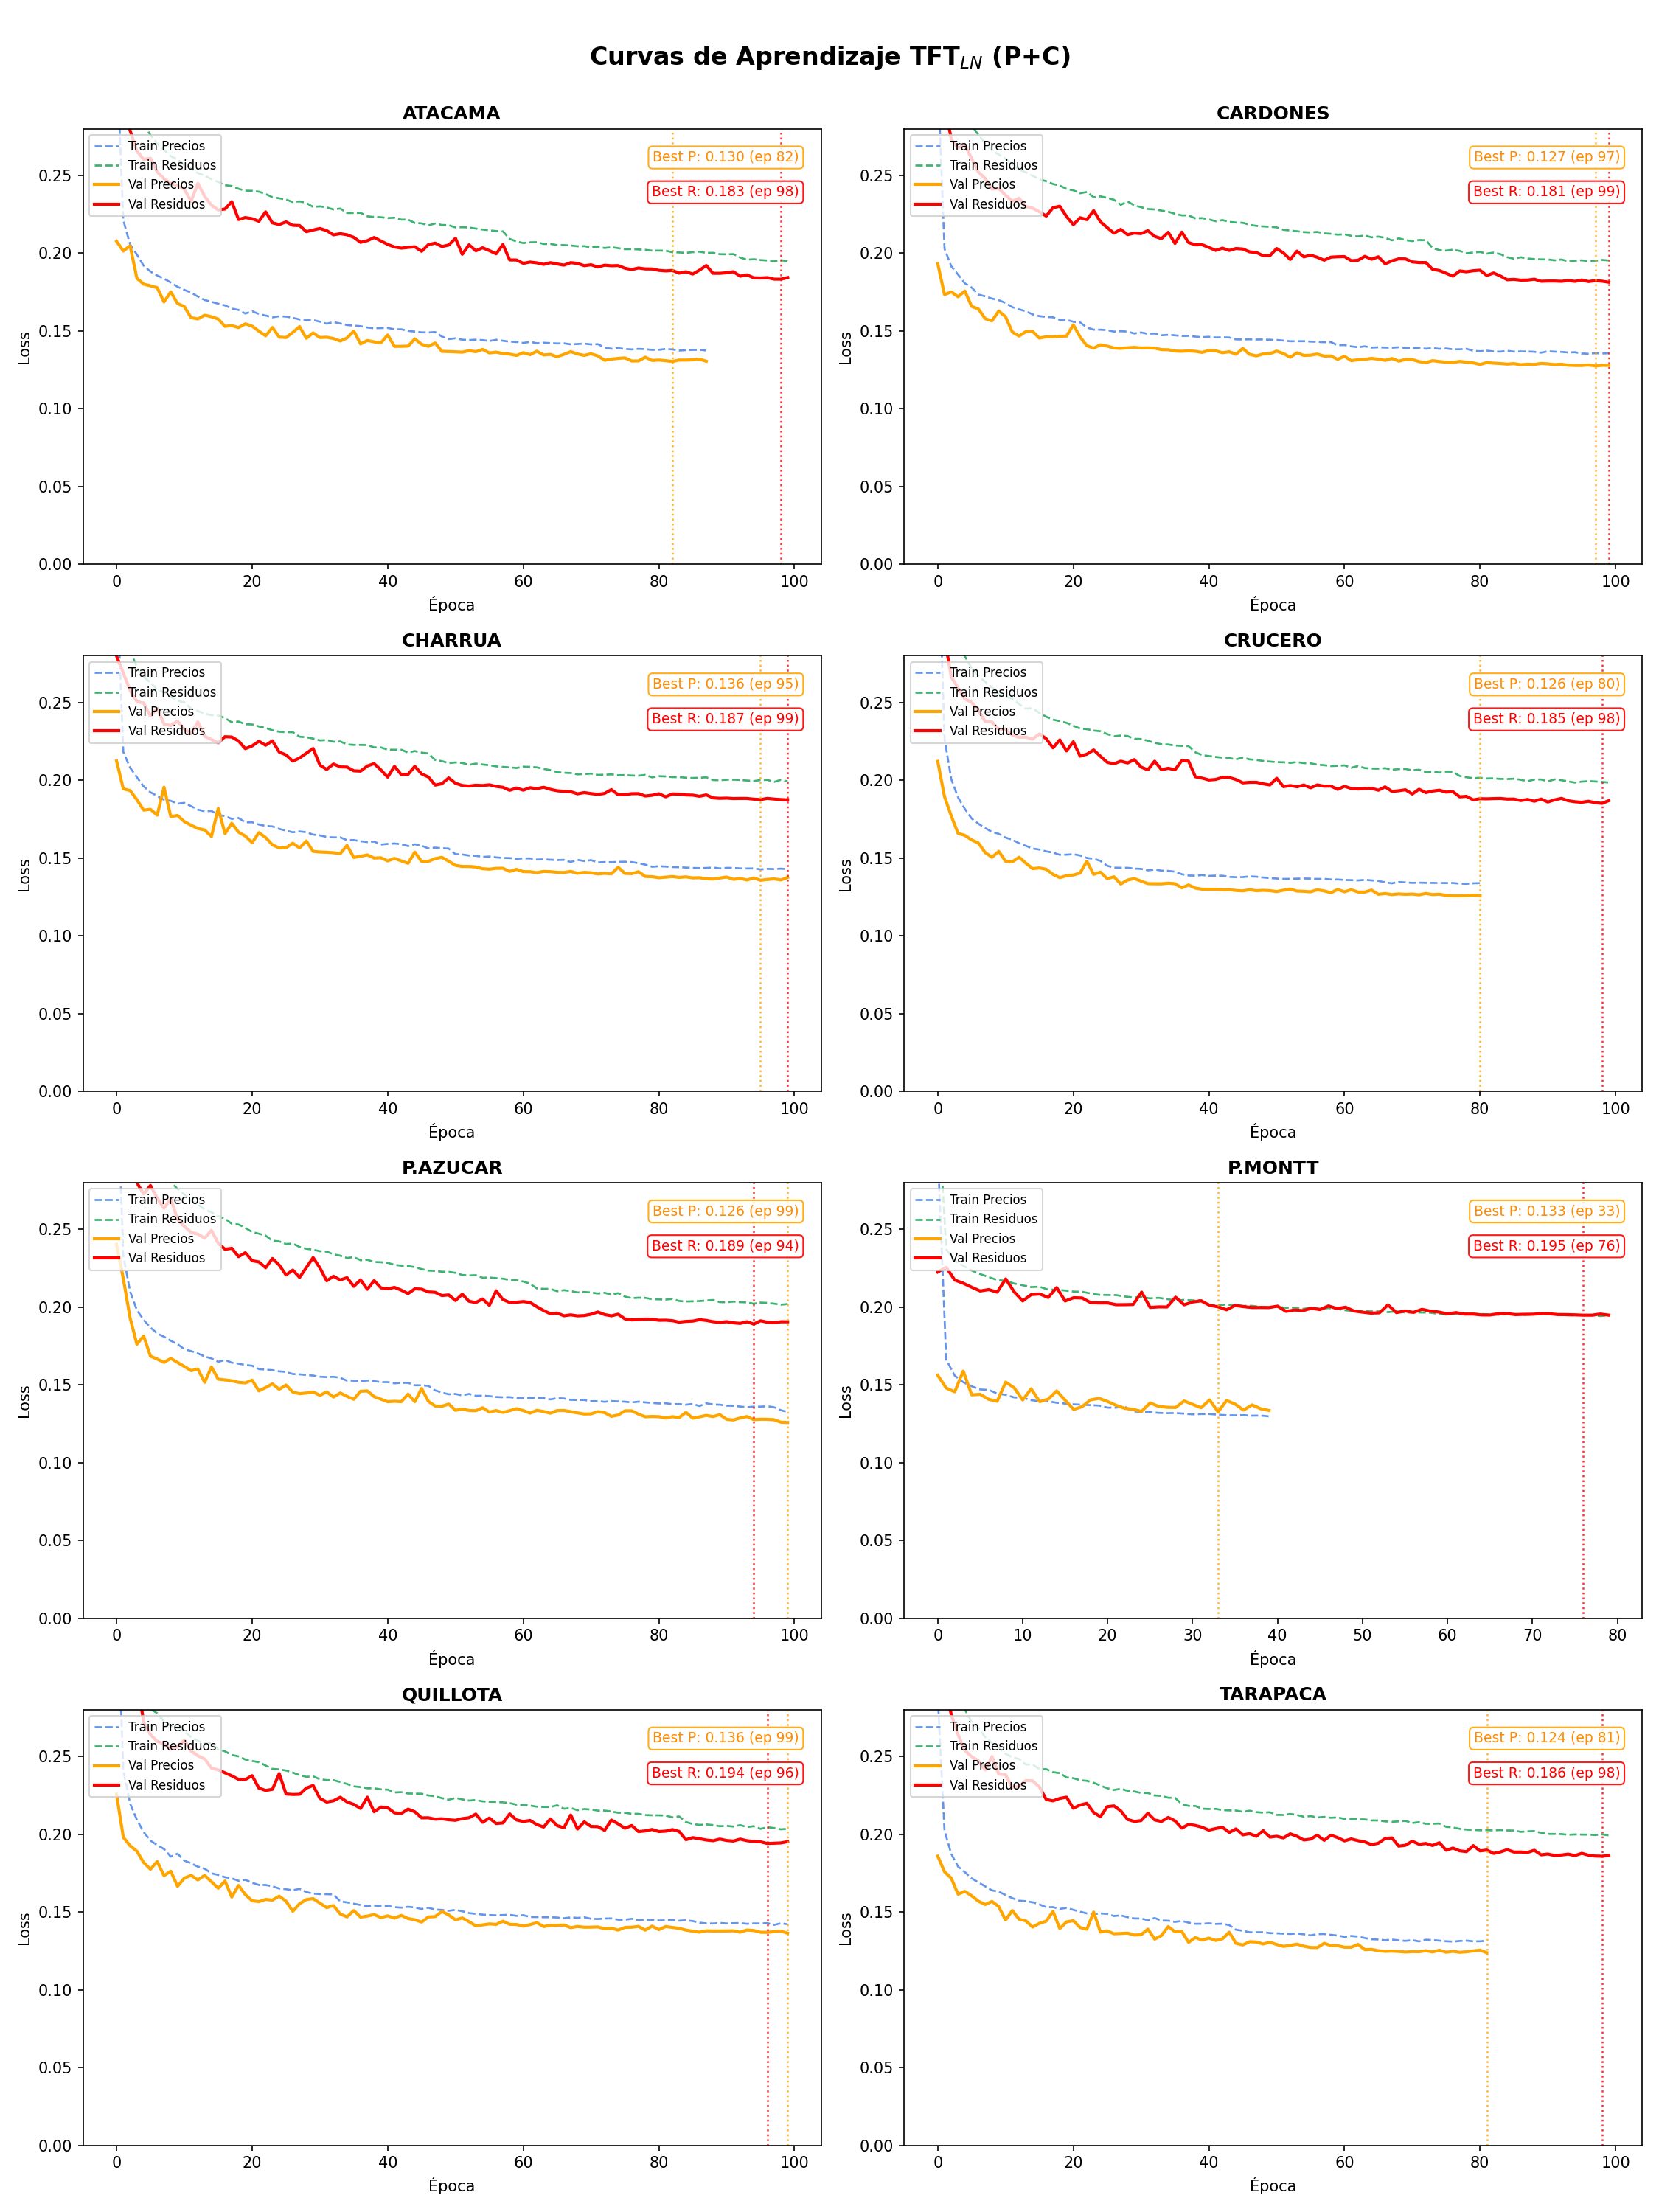
\includegraphics[width=0.95\textwidth]{imagenes/Posibles img/Curvas Aprendizaje LN.png}
    \caption{Curvas de aprendizaje del TFT con LayerNorm para las ocho barras del SEN. Se muestran la pérdida (MAE) de entrenamiento y validación para los modelos de precios y residuos. Las líneas verticales indican la época de mejor desempeño en validación.}
    \label{fig:tft_learning_curves}
\end{figure}

Las curvas muestran convergencia estable en la mayoría de las barras sin señales de sobreajuste severo. La pérdida de validación del modelo de precios converge en torno a 0.124--0.136, mientras que la del modelo de residuos se estabiliza alrededor de 0.181--0.195, lo que es esperable dado que los residuos de Prophet son intrínsecamente más difíciles de predecir que la serie original al haber eliminado la estructura sistemática de largo plazo. La mayoría de los modelos alcanza su mejor desempeño en épocas avanzadas del entrenamiento (entre las épocas 80 y 99), lo que indica que el límite de 100 épocas es adecuado y que el early stopping no se activa prematuramente; Puerto Montt es la excepción, con el modelo de precios deteniéndose de forma más temprana (mejor época 33), consistente con la mayor volatilidad estructural de esta barra ya documentada en la Sección 3.1.

\section{Stacking Optimization}

\subsection{Estrategias de ensamblaje}

El Stacking Optimization combina las predicciones de Prophet y las dos instancias del TFT mediante una combinación lineal convexa con pesos aprendidos sobre el conjunto de validación, siguiendo el marco descrito en la Sección 2.5. Se evalúan seis estrategias de ensamblaje que cubren desde los modelos base individuales hasta combinaciones progresivamente más complejas:

\begin{enumerate}
    \item \textbf{Prophet solo:} predicción directa de Prophet sin combinación.
    \item \textbf{$\text{TFT}_\text{LN}$ precios solo:} predicción directa del TFT entrenado sobre la serie de precios.
    \item \textbf{Prophet $+$ $\text{TFT}_\text{LN}$ precios:} combinación convexa $\hat{y} = w_1 \hat{y}^{\text{Prophet}} + w_2 \hat{y}^{\text{TFT}_\text{P}}$.
    \item \textbf{Prophet $+$ $\text{TFT}_\text{LN}$ residuos (D):} suma directa $\hat{y} = \hat{y}^{\text{Prophet}} + \hat{r}^{\text{TFT}_\text{R}}$ con pesos fijos $w_1 = w_2 = 1$.
    \item \textbf{Prophet $+$ $\text{TFT}_\text{LN}$ residuos (Opt):} combinación convexa $\hat{y} = w_1 \hat{y}^{\text{Prophet}} + w_2 \hat{r}^{\text{TFT}_\text{R}}$ con pesos optimizados.
    \item \textbf{(Prophet $+$ residuos) $+$ $\text{TFT}_\text{LN}$ precios (opt):} combinación convexa entre la predicción híbrida Prophet-residuos con suma directa y el $\text{TFT}_\text{LN}$ de precios, $\hat{y} = w_1 (\hat{y}^{\text{Prophet}} + \hat{r}^{\text{TFT}_\text{R}}) + w_2 \hat{y}^{\text{TFT}_\text{P}}$, con pesos optimizados.
\end{enumerate}

En todas las estrategias con optimización de pesos se impone la restricción de combinación convexa $w_1 + w_2 = 1$ con $w_1, w_2 \geq 0$, de modo que los pesos son interpretables como cuotas de participación de cada componente. Los pesos se estiman minimizando el MAE sobre el conjunto de validación y se aplican sin reestimación al conjunto de prueba.

\subsection{Métodos de optimización de pesos}

Para las estrategias que requieren optimización de pesos se comparan ocho métodos numéricos sobre el mismo problema de un grado de libertad ($w_1$, con $w_2 = 1 - w_1$): búsqueda en grilla con resoluciones de 21, 41 y 101 puntos (\textit{Grid\_21}, \textit{Grid\_41}, \textit{Grid\_101}), Nelder-Mead, SLSQP, L-BFGS-B, Evolución Diferencial y búsqueda aleatoria con 1.000 iteraciones (\textit{Random\_1000}), más Regresión Ridge ($\alpha = 0.01$) como comparación aparte: Ridge no optimiza la misma función objetivo MAE, sino que resuelve en forma cerrada un problema distinto (mínimos cuadrados con penalización $\ell_2$), por lo que se incluye para verificar que un estimador de uso común no se aleja del óptimo de los ocho anteriores, no como un noveno método sobre el mismo problema. Todos optimizan sobre el conjunto de validación y los pesos resultantes se evalúan en prueba sin reajuste.

Como se muestra en la Sección 4.3.1, la elección de método resulta irrelevante para la calidad del resultado final: al ser la función objetivo MAE convexa y unimodal en una variable, los ocho métodos numéricos convergen esencialmente al mismo mínimo, con diferencias inferiores al 0.1\%, y Ridge tampoco se aparta de ese óptimo de forma apreciable pese a resolver un problema distinto. La diferencia práctica entre métodos es el tiempo de cómputo, irrelevante a esta escala (SLSQP y Ridge bajo 0.05\,s en la mayoría de las barras; la búsqueda aleatoria, la más lenta, 0.5--1.2\,s); los resultados reportados en el resto de este trabajo emplean indistintamente el método con menor MAE de cada barra y estrategia.

\section{TFT con Dynamic Tanh}

El $\text{TFT}_\text{DyT}$ es una variante del TFT con LayerNorm descrito en la Sección 3.4 en la que todas las capas LayerNorm de la arquitectura son reemplazadas por capas Dynamic Tanh (DyT), siguiendo la sustitución uniforme descrita en la Sección 2.4.5. La configuración de features, dataloaders, hiperparámetros y protocolo de entrenamiento es idéntica a la del $\text{TFT}_\text{LN}$, con la única diferencia en el mecanismo de normalización. El parámetro $\alpha$ de cada capa DyT se inicializa en $\alpha_0 = 0.5$ con $\boldsymbol{\gamma} = \mathbf{1}$ y $\boldsymbol{\beta} = \mathbf{0}$, siguiendo la recomendación de Zhu et al. (2025) para modelos no-LLM descrita en la Sección 2.4.3. El mismo esquema de Stacking Optimization descrito en la Sección 3.5, con las seis estrategias de ensamblaje y los ocho métodos numéricos de optimización de pesos más Ridge, se aplica de forma idéntica sobre las predicciones del $\text{TFT}_\text{DyT}$, sustituyendo únicamente las predicciones puntuales de entrada por las del modelo con DyT.

\subsection{Curvas de aprendizaje}

La Figura \ref{fig:dyt_learning_curves} presenta las curvas de aprendizaje del $\text{TFT}_\text{DyT}$ para las ocho barras del SEN.

\begin{figure}[htbp]
    \centering
    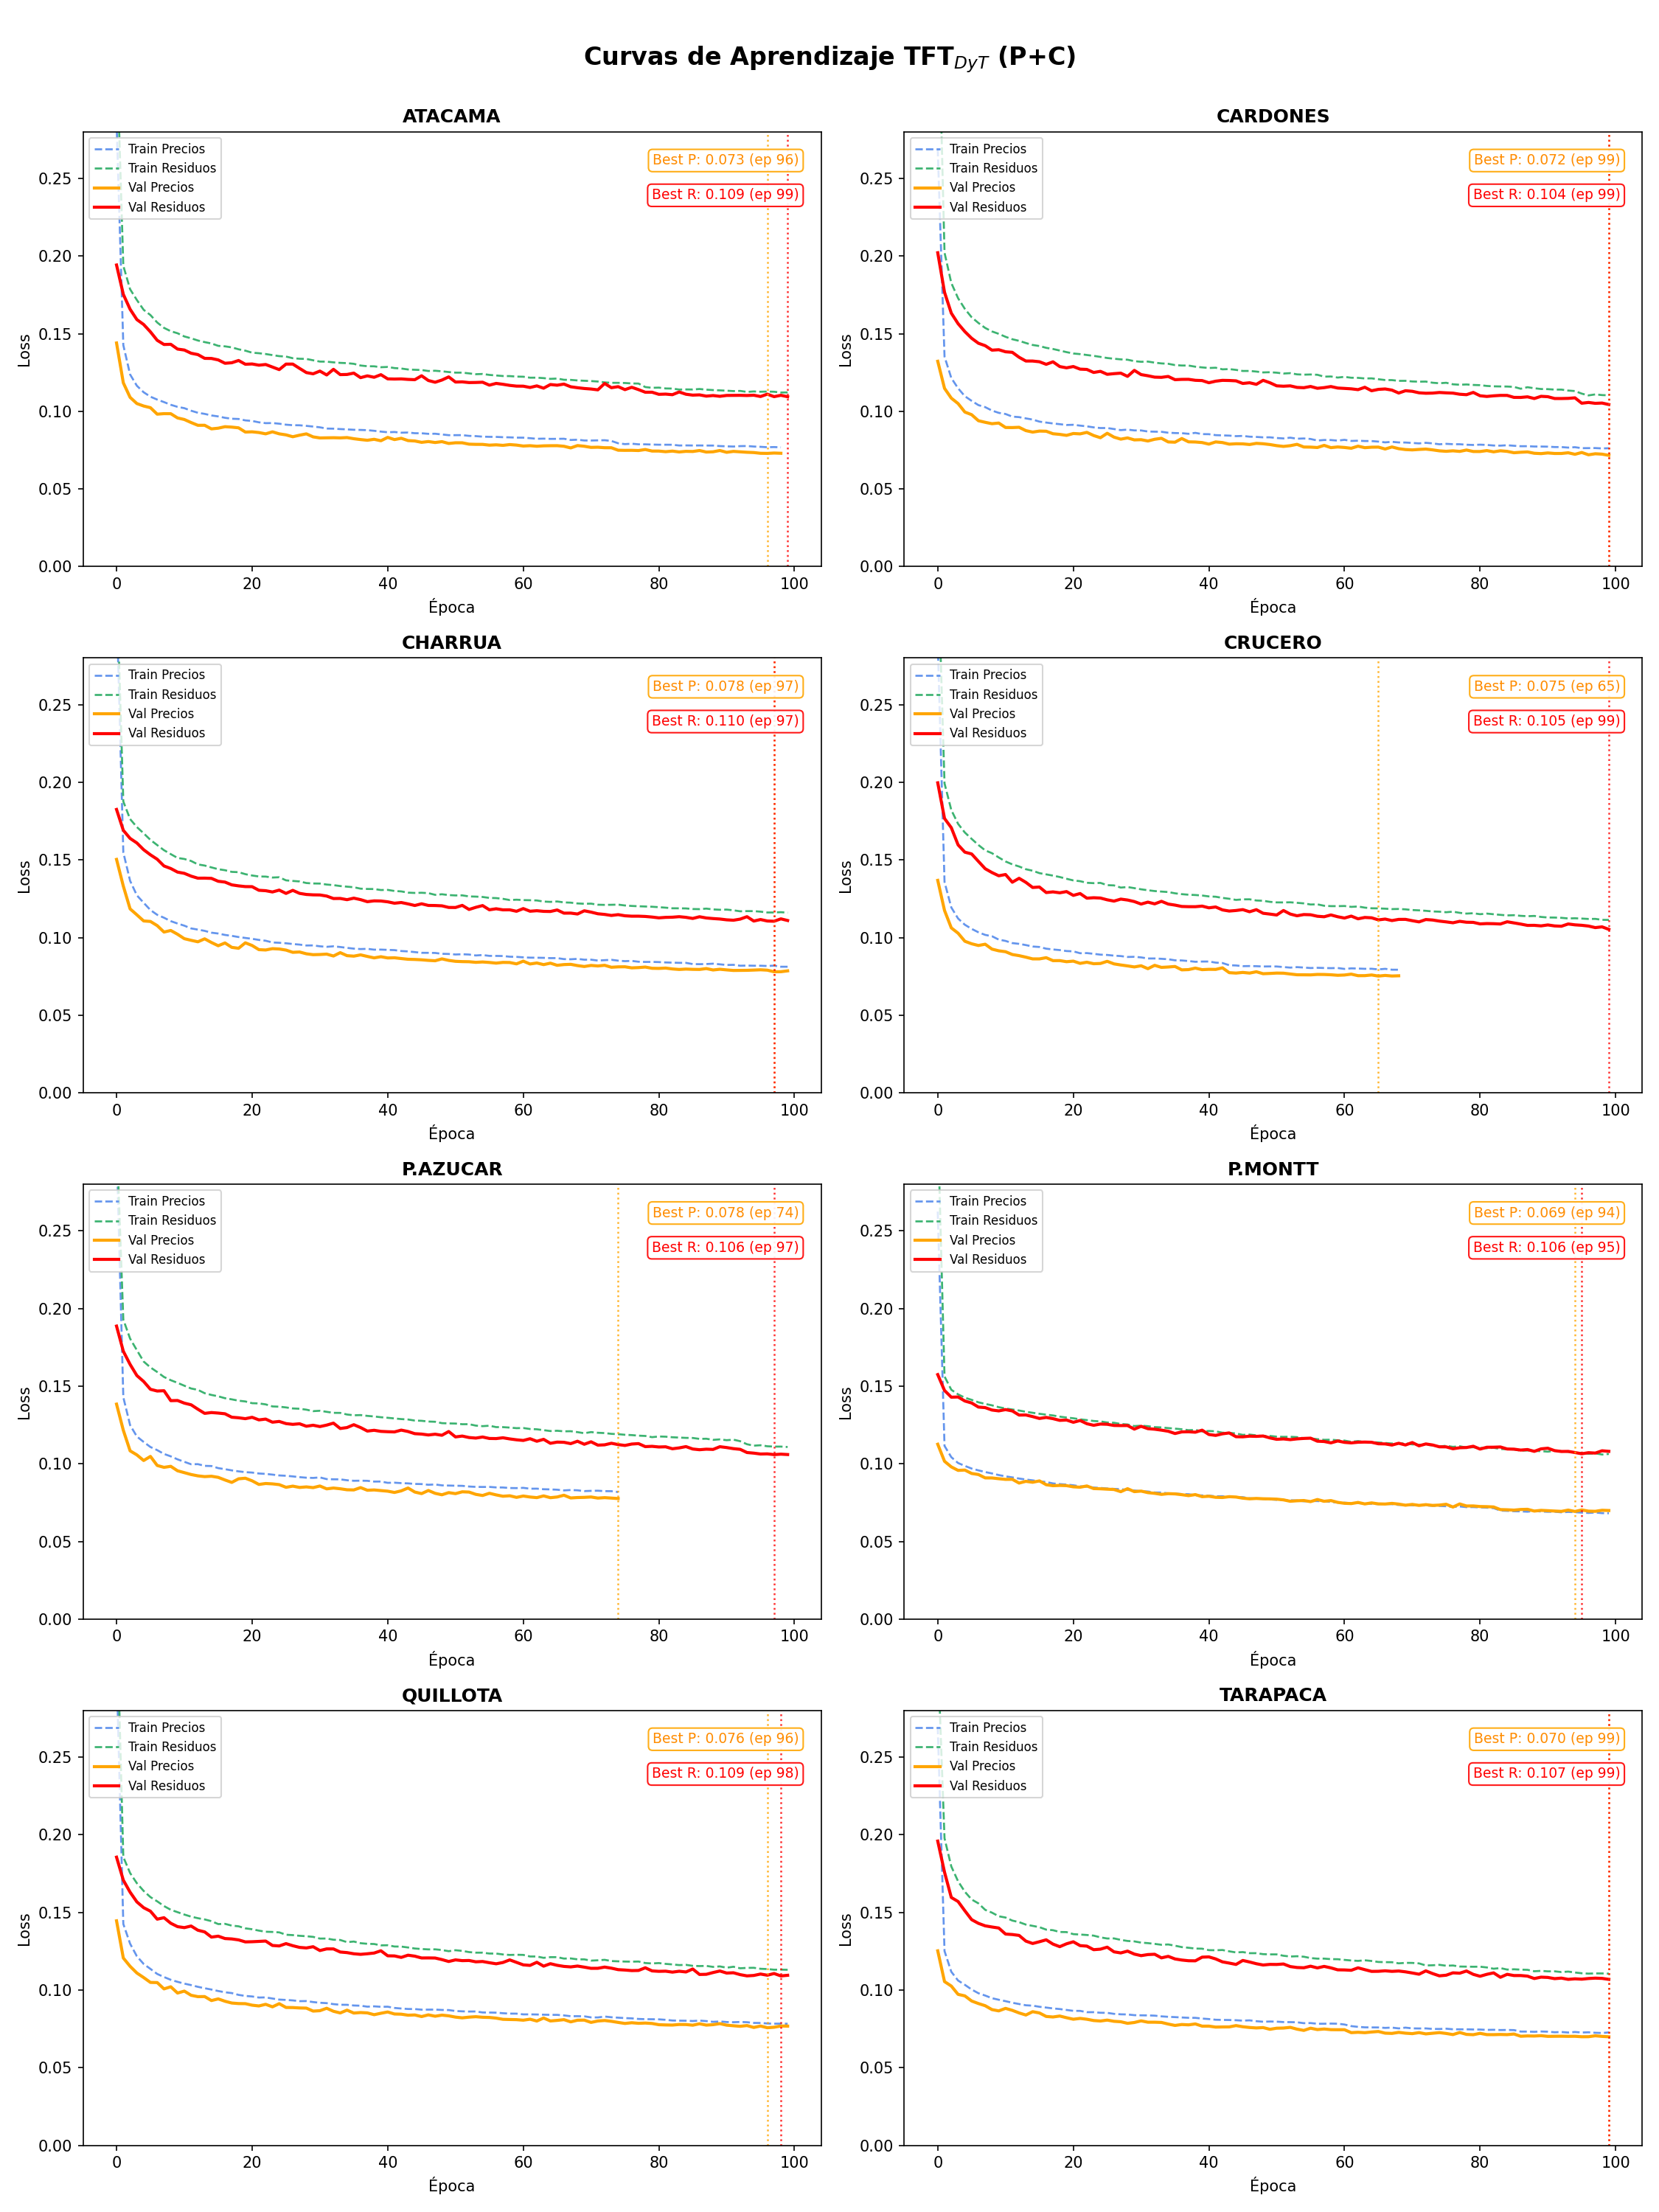
\includegraphics[width=0.95\textwidth]{imagenes/Posibles img/Curvas Aprendizaje DyT.png}
    \caption{Curvas de aprendizaje del TFT con DyT para las ocho barras del SEN. Se muestran la pérdida (MAE) de entrenamiento y validación para los modelos de precios y residuos. Las líneas verticales indican la época de mejor desempeño en validación.}
    \label{fig:dyt_learning_curves}
\end{figure}

Al igual que con $\text{TFT}_\text{LN}$, las curvas muestran una convergencia estable sin señales de sobreajuste severo: la pérdida de entrenamiento y de validación decrecen de forma conjunta y se estabilizan hacia el final del entrenamiento, sin la divergencia creciente entre ambas que caracterizaría al sobreajuste. La pérdida de validación del modelo de precios converge en torno a 0.069--0.078, y la del modelo de residuos alrededor de 0.104--0.110. La mayoría de los modelos alcanza su mejor desempeño en épocas avanzadas del entrenamiento, mayoritariamente entre las épocas 94 y 99, con algunas excepciones que se estabilizan algo antes (Crucero, precios, época 65).

\subsection{\texorpdfstring{Análisis del parámetro $\alpha$ aprendido}{Análisis del parámetro alfa aprendido}}

La Figura \ref{fig:alpha_dyt} presenta los valores del parámetro $\alpha$ aprendido por cada capa DyT del $\text{TFT}_\text{DyT}$, agrupados por módulo de la arquitectura. La línea roja punteada indica el valor de inicialización $\alpha_0 = 0.5$.

\begin{figure}[htbp]
    \centering
    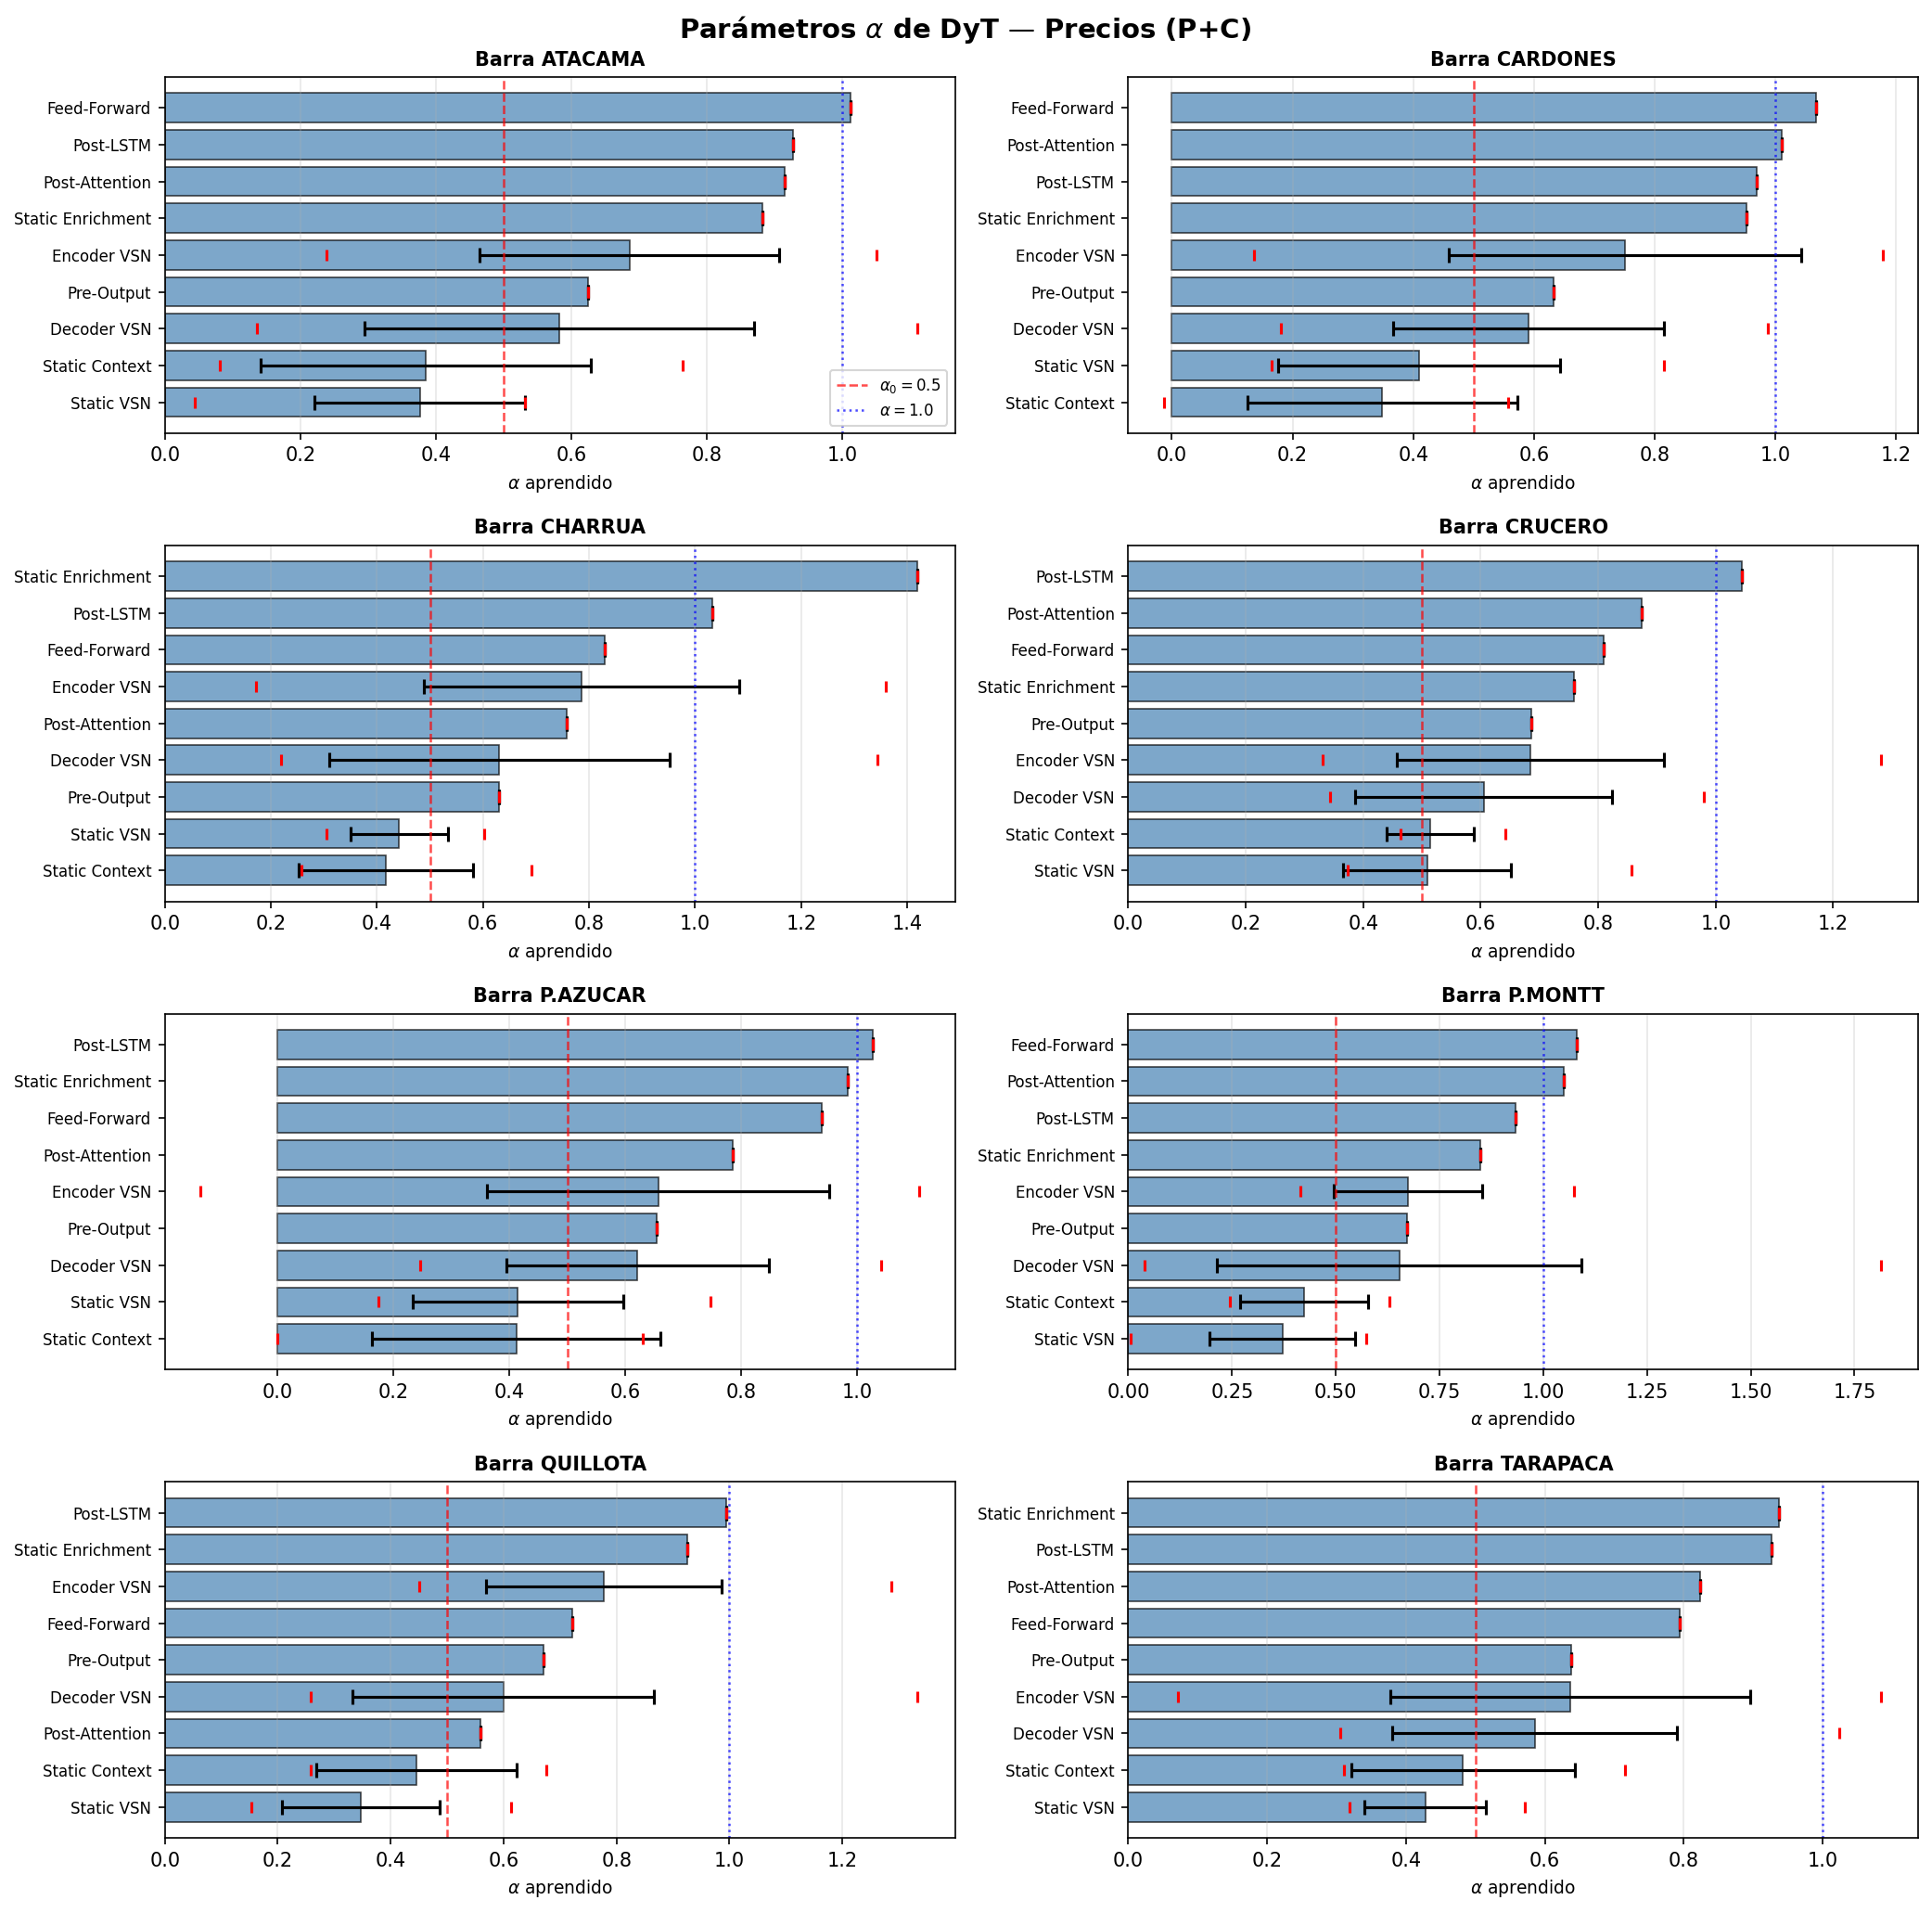
\includegraphics[width=0.85\textwidth]{imagenes/Posibles img/Alphas Aprendidos Precios.png}
    \caption{Valores del parámetro $\alpha$ aprendido por las capas DyT del $\text{TFT}_\text{DyT}$ para las ocho barras del SEN, agrupados por módulo de la arquitectura. Las barras muestran la media por módulo, las líneas de error la desviación estándar, y los marcadores rojos el mínimo y máximo. La línea roja punteada indica el valor de inicialización $\alpha_0 = 0.5$.}
    \label{fig:alpha_dyt}
\end{figure}

El resultado central de este análisis es que los valores de $\alpha$ se dispersaron significativamente desde el valor de inicialización $\alpha_0 = 0.5$, cubriendo un rango de $-0.13$ a $1.81$ al final del entrenamiento, con algunas capas individuales incluso aprendiendo valores levemente negativos lo que sigue siendo una transformación válida, dado que $\tanh$ es una función impar y un $\alpha$ negativo solo invierte la polaridad de esa unidad de squashing. Esto confirma que DyT efectivamente aprendió a normalizar de manera adaptativa durante el entrenamiento, en lugar de mantener una compresión fija, tal como predice la teoría de Zhu et al. (2025). Los módulos de selección de variables, Encoder VSN, Decoder VSN y Static VSN, presentan mayor dispersión entre capas que los módulos de más alto nivel como Feed-Forward y Post-LSTM, lo que refleja la heterogeneidad entre las features procesadas en cada módulo.

\subsection{Curvas de aprendizaje de S+C}

La Figura \ref{fig:sc_learning_curves} presenta las curvas de aprendizaje de la rama S+C para las ocho barras del SEN, comparando directamente $\text{TFT}_\text{LN}$ y $\text{TFT}_\text{DyT}$ sobre el único modelo que entrena esta rama, sin residuos de Prophet (Sección 3.4.1).

\begin{figure}[htbp]
    \centering
    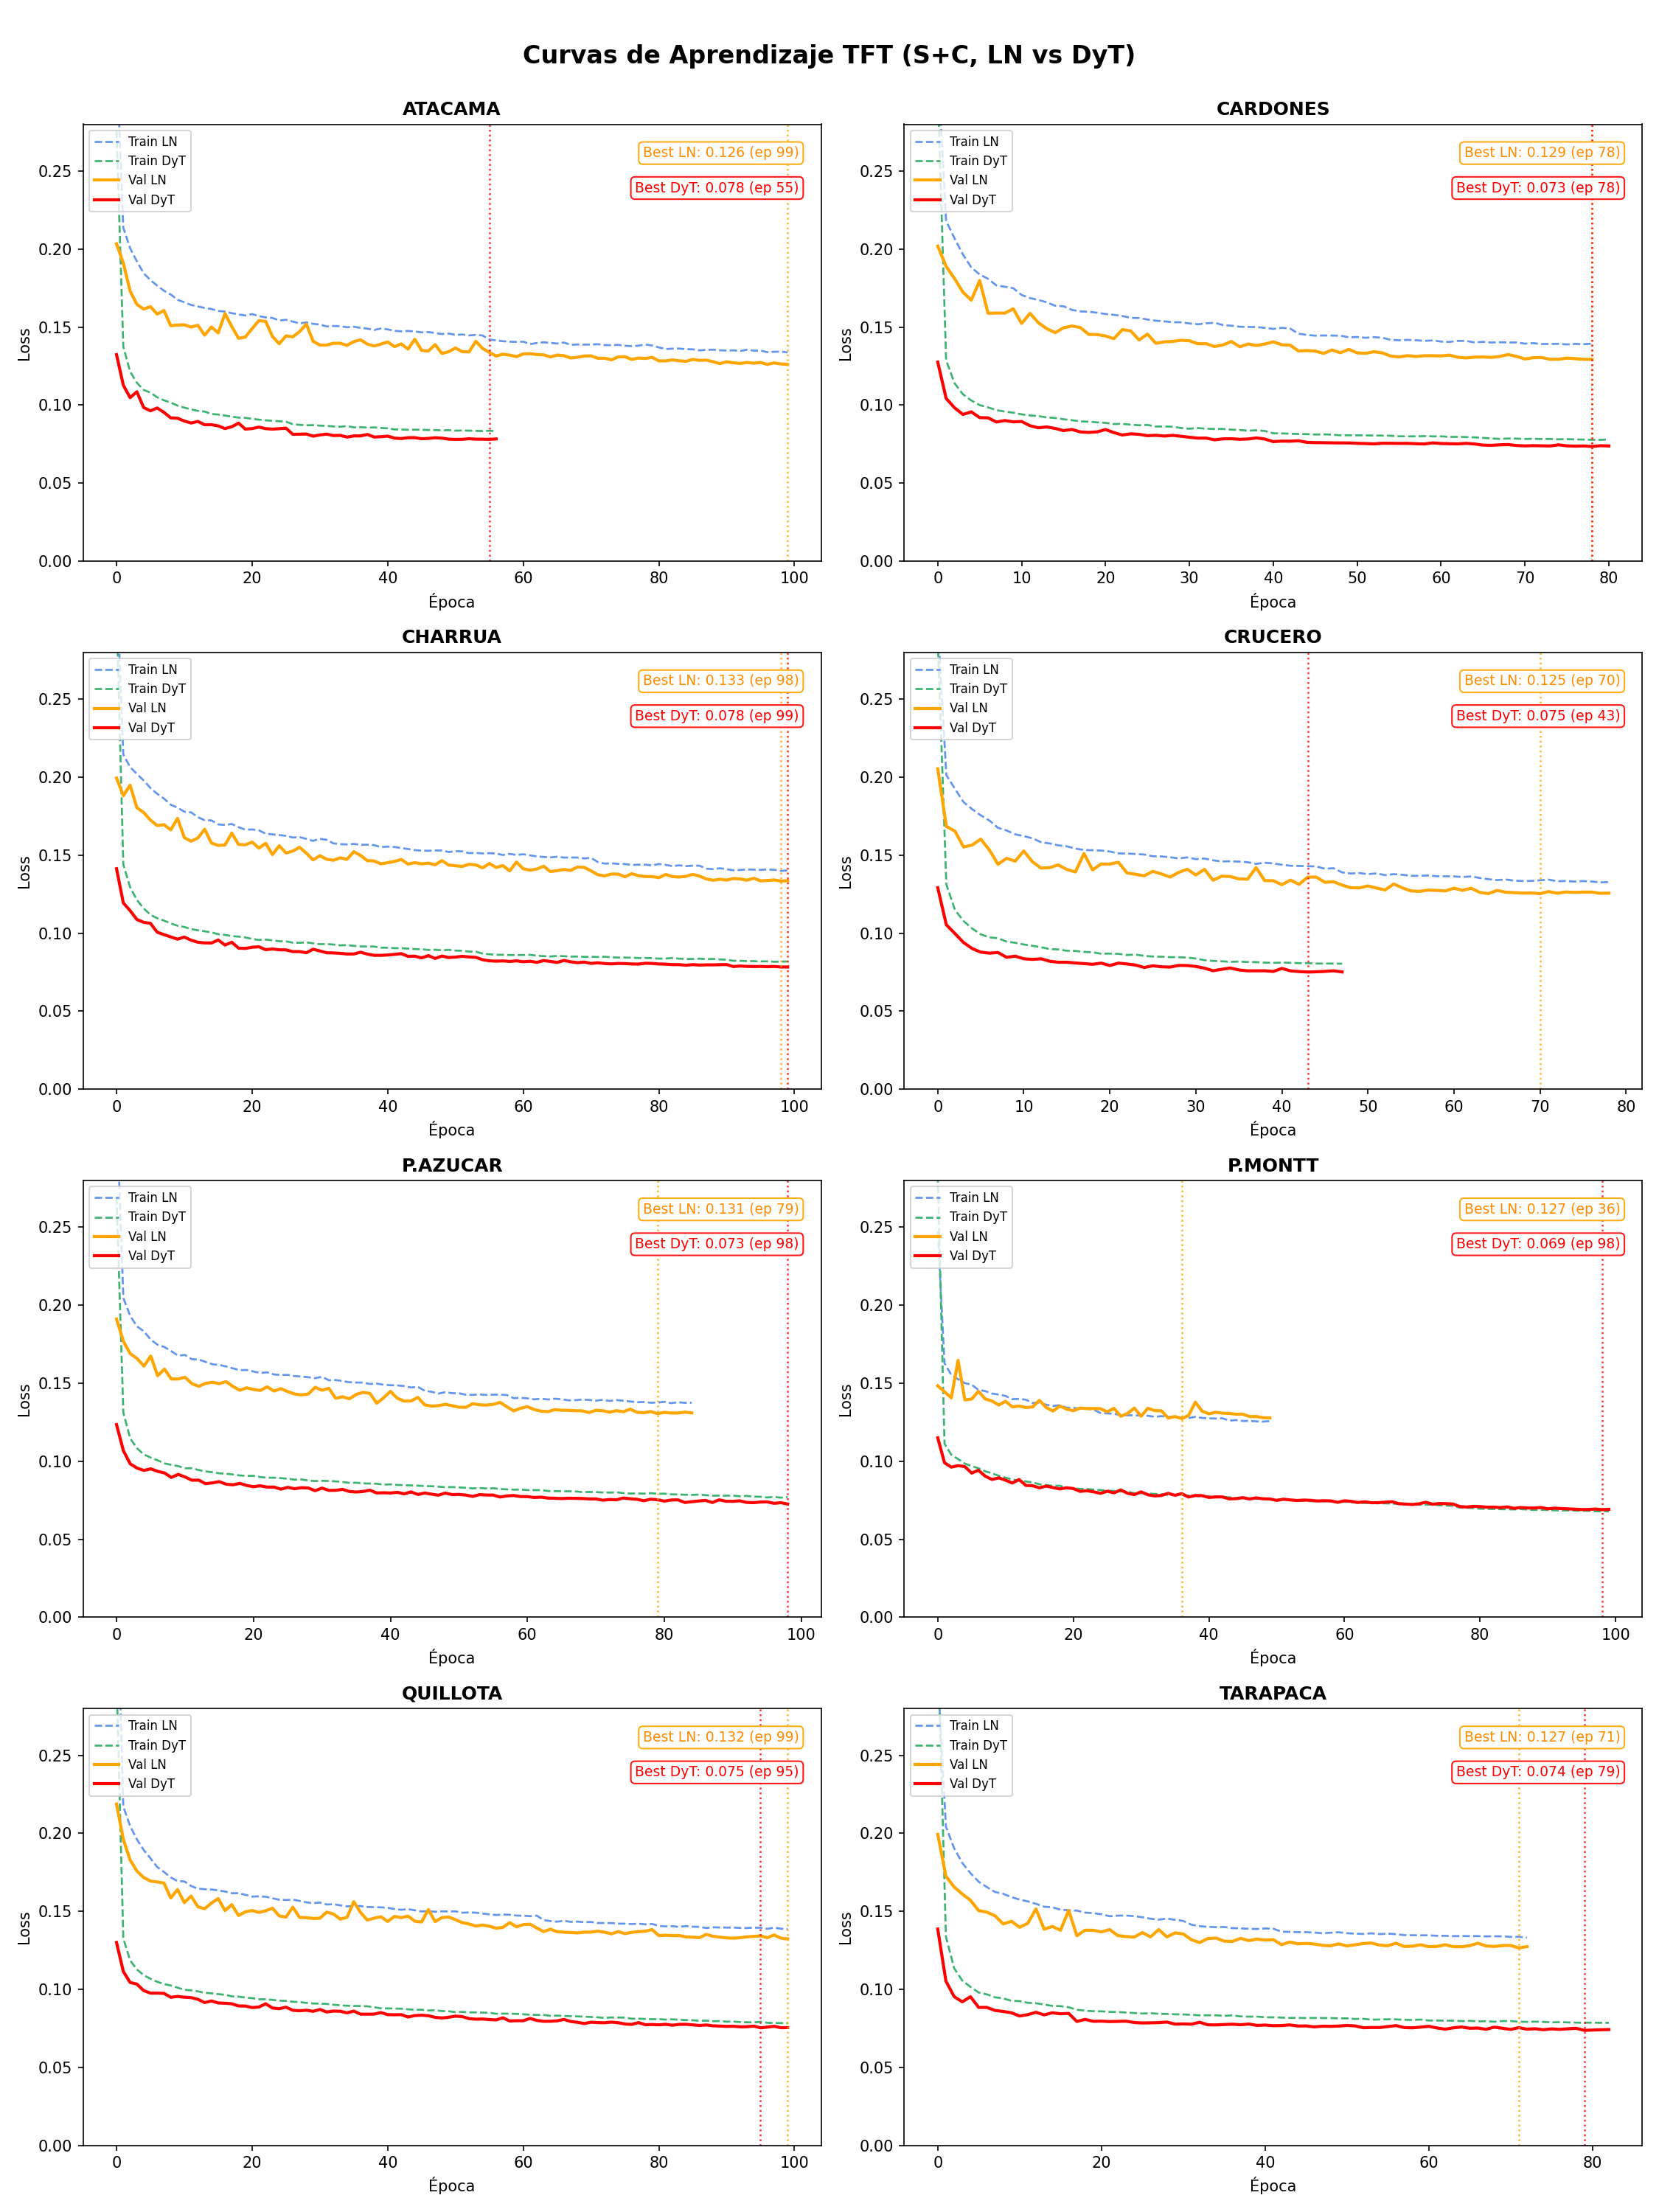
\includegraphics[width=0.95\textwidth]{imagenes/Posibles img/Curvas Aprendizaje SC.png}
    \caption{Curvas de aprendizaje de la rama S+C para las ocho barras del SEN, comparando $\text{TFT}_\text{LN}$ y $\text{TFT}_\text{DyT}$. Se muestra la pérdida (MAE) de entrenamiento y validación. Las líneas verticales indican la época de mejor desempeño en validación.}
    \label{fig:sc_learning_curves}
\end{figure}

Al igual que en P+C, ambas arquitecturas muestran convergencia estable sin señales de sobreajuste en S+C. La pérdida de validación de $\text{TFT}_\text{LN}$ converge en torno a 0.125--0.133, y la de $\text{TFT}_\text{DyT}$ alrededor de 0.069--0.078, magnitudes consistentes con las observadas en P+C (Secciones 3.4.3 y 3.6.1) para cada arquitectura respectivamente. La mayoría de los modelos alcanza su mejor desempeño en épocas avanzadas del entrenamiento, aunque con mayor variabilidad entre barras que en P+C; Puerto Montt es nuevamente el caso más temprano ($\text{TFT}_\text{LN}$, época 36), consistente con su mayor volatilidad estructural ya documentada en la Sección 3.1.

\section{Conformal Prediction}

La Predicción Conforme se aplica sobre la predicción puntual de S+C-LN, la estrategia de referencia seleccionada en la Sección 4.4.5, con el objetivo de construir intervalos de cobertura garantizada para cada barra. En esta sección se describe la configuración del esquema de calibración y las cinco variantes implementadas sobre S+C-LN, más CQR como comparación externa; los resultados se presentan en el Capítulo 4.

\subsection{Configuración general}
\label{sec:cp_configuracion_general}

Todas las variantes se evalúan con nivel de cobertura nominal $1 - \alpha = 0.95$ y operan sobre la escala original de los costos marginales en USD/MWh. El conjunto de calibración es el conjunto de validación descrito en la Tabla \ref{tab:division}, que cubre el período junio 2024--mayo 2025 con $n_{\text{cal}} = 8\,298$ observaciones por barra; el conjunto de evaluación es el conjunto de prueba, con $n_{\text{test}} = 8\,298$ observaciones horarias por barra, cubriendo mayo 2025--abril 2026. Se excluye del conjunto de calibración una ventana de 11 horas (25--26 de febrero de 2025) en la que las ocho barras registraron simultáneamente el mismo valor exacto (576.82\,USD/MWh): un precio de falla administrativo aplicado uniformemente a todo el sistema, no un precio de mercado dependiente de las variables que el modelo puntual utiliza como predictores (Sección \ref{sec:split_cp_clasico}). El límite inferior de todos los intervalos, sin excepción, se trunca en 0 USD/MWh para respetar el dominio físico del costo marginal; el truncamiento no altera la cobertura empírica reportada, solo reduce el ancho medio en la magnitud correspondiente a la porción del intervalo que caía por debajo de 0 antes de truncar (Sección \ref{sec:split_cp_clasico}).

Los \textit{scores} de no conformidad utilizados en todas las variantes son los residuos absolutos del modelo de predicción puntual:

\begin{equation}
    s_t = \lvert y_t - \hat{y}_t \rvert,
    \label{eq:nonconformity}
\end{equation}

donde $\hat{y}_t$ es la predicción puntual cruda de S+C-LN para la barra correspondiente, la misma para las cinco variantes implementadas: usar un único predictor puntual es necesario para que el ancho de intervalo resultante sea comparable entre métodos (Sección \ref{sec:lwacp_comparativa}), ya que cambiar el modelo base de un método a otro confundiría el efecto propio de cada mecanismo de calibración con el efecto de un predictor distinto. Los intervalos resultantes son simétricos alrededor de $\hat{y}_t$:

\begin{equation}
    C_t = \bigl[\,\hat{y}_t - q_t,\; \hat{y}_t + q_t\,\bigr],
    \label{eq:interval}
\end{equation}

donde $q_t$ es el cuantil adaptado por cada método en el instante $t$. Las métricas de evaluación son la cobertura empírica (\textit{Coverage}), el ancho medio del intervalo (\textit{Width}) y el MAE de la predicción puntual subyacente.

Cabe señalar una limitación metodológica del esquema de calibración adoptado. El conjunto de validación cumple un doble rol: primero, participa en la selección del punto de early-stopping del entrenamiento del TFT (Sección 3.4.2); segundo, se utiliza como conjunto de calibración para estimar el cuantil de no conformidad. Esto puede producir un cuantil $q$ ligeramente subestimado respecto al que se obtendría sobre datos completamente independientes, ya que el modelo fue implícitamente seleccionado para desempeñarse bien sobre ese mismo conjunto. La solución ideal sería un tercer conjunto dedicado exclusivamente a calibración, pero con datos de series de tiempo esto reduce el tamaño de calibración disponible. Con $n_{\text{cal}} = 8\,298$ observaciones el sesgo es probablemente pequeño dado el tamaño del conjunto, y se reporta como limitación del diseño experimental.

\subsection{Split CP clásico}

El Split CP clásico, descrito en la Sección 2.6.1, calcula un cuantil fijo $q$ a partir del conjunto de calibración y lo aplica sin cambios a todo el período de prueba. Formalmente, dados los \textit{scores} de calibración $\{s_i\}_{i=1}^{n_{\text{cal}}}$ definidos en \eqref{eq:nonconformity}, el cuantil se obtiene como

\begin{equation}
    q = \hat{Q}_{1-\alpha}\!\left(\{s_i\}_{i=1}^{n_{\text{cal}}}\right),
    \quad
    \text{con nivel ajustado }
    \frac{\lceil (1-\alpha)(n_{\text{cal}}+1)\rceil}{n_{\text{cal}}+1},
    \label{eq:scp_quantile}
\end{equation}

garantizando cobertura marginal finita cuando las observaciones son intercambiables (Vovk et al., 2005) \cite{VovkCP}.

\subsection{ACI}
\label{sec:aci_metodologia}

La \textit{Adaptive Conformal Inference} (ACI), propuesta por Gibbs y Candès (2021) y descrita en la Sección 2.6.4, adapta el nivel de cobertura efectivo $\alpha_t$ en cada instante según la historia reciente de errores de cobertura, sin modificar el \textit{score} de no conformidad ni el modelo de predicción puntual, que es el mismo $\hat{y}_t$ de S+C-LN usado por Split CP, LW Split CP y LW-ACP. El nivel evoluciona según la regla de actualización

\begin{equation}
    \alpha_{t+1} = \alpha_t + \gamma\,(\alpha - \mathbf{1}_{\{y_t \notin C_t\}}),
    \label{eq:aci_update_metodologia}
\end{equation}

donde $\gamma = 0.05$, fijado de antemano e igual al usado en LW-ACP (Sección \ref{sec:lwacp}), en vez de compararse varios valores de $\gamma$ y reportar el de mejor desempeño en el conjunto de prueba; $\alpha = 0.05$ es el nivel nominal. Formalmente, en cada paso $t$ del conjunto de prueba: se calcula el cuantil $q_t$ de los \textit{scores} de calibración con nivel $1-\alpha_t$, se construye $C_t = [\hat{y}_t - q_t,\, \hat{y}_t + q_t]$, se observa $y_t$ y se actualiza $\alpha_{t+1}$ según \eqref{eq:aci_update_metodologia}. Al no reajustarse ningún modelo de predicción en cada paso --solo el escalar $\alpha_t$--, ACI no distingue entre una variante \textit{offline} y una \textit{online} como en formulaciones que sí incorporan un modelo auxiliar reentrenable: es un único método, con un costo computacional equivalente al de Split CP más la actualización escalar de $\alpha_t$ en cada instante.

\subsection{LW Split CP}

La \textit{Locally-Weighted Split CP} (LW Split CP), descrita en la Sección \ref{sec:lwacp}, reemplaza el score de no conformidad absoluto \eqref{eq:nonconformity} por su versión normalizada por hora del día:

\begin{equation}
    \tilde{s}_i = \frac{s_i}{\hat{\sigma}_{h(i)}}, \qquad i \in \mathcal{C}al
    \label{eq:lw_score_metodologia}
\end{equation}

donde $\hat{\sigma}_h$ es la desviación estándar de los residuos absolutos de calibración de la hora $h$, estimada según \eqref{eq:sigma_h} con un mínimo de 30 observaciones por hora; si alguna hora no alcanza ese mínimo, se usa la desviación estándar global de calibración como respaldo. Con $n_{\text{cal}} = 8\,298$ observaciones repartidas en 24 horas, cada hora dispone en promedio de $346$ observaciones, muy por sobre el umbral mínimo. Adicionalmente, $\hat{\sigma}_h$ se acota inferiormente por la desviación estándar global de calibración ($\hat{\sigma}_h \geq \hat{\sigma}_{\text{global}}$): sin este piso, en horas de variabilidad intrínsecamente baja un único \textit{score} de calibración inusualmente grande, al normalizarse por un $\hat{\sigma}_h$ casi nulo, produce un \textit{score} normalizado extremo que infla el cuantil $q$ para todas las horas, no solo la afectada --efecto verificado empíricamente en dos de las ocho barras (Sección \ref{sec:lw_split_cp})--. El cuantil $q$ se calcula sobre los scores normalizados $\{\tilde{s}_i\}$ con la misma corrección de muestra finita de \eqref{eq:scp_quantile}, y el intervalo en cada instante de prueba se reescala por la desviación local de esa hora: $C_t = [\hat{y}_t - q\,\hat{\sigma}_{h(t)},\; \hat{y}_t + q\,\hat{\sigma}_{h(t)}]$.

\subsection{LW-ACP Online}

La \textit{Locally-Weighted Adaptive Conformal Prediction} (LW-ACP), descrita en la Sección \ref{sec:lwacp}, combina la normalización por hora de \eqref{eq:lw_score_metodologia} con la actualización online del nivel de cobertura de ACI \eqref{eq:aci_update_metodologia}. El conjunto de scores normalizados de calibración $\{\tilde{s}_i\}_{i \in \mathcal{C}al}$ se calcula una única vez, igual que en LW Split CP; lo que varía en cada paso $t$ del conjunto de prueba es el nivel de cobertura efectivo $\alpha_t$, que determina un cuantil distinto en cada instante:

\begin{equation}
    q_t = \hat{Q}_{1-\alpha_t}\!\left(\{\tilde{s}_i\}_{i \in \mathcal{C}al}\right), \qquad
    C_t = \left[\hat{y}_t - q_t\,\hat{\sigma}_{h(t)},\; \hat{y}_t + q_t\,\hat{\sigma}_{h(t)}\right]
\end{equation}

Tras observar $y_t$, se actualiza $\alpha_{t+1} = \alpha_t + \gamma\,(\alpha - \mathbf{1}_{\{y_t \notin C_t\}})$, con $\alpha_{t+1}$ acotado al intervalo $[0.001,\, 0.999]$ para evitar niveles degenerados. Se utiliza $\gamma = 0.05$, fijado de antemano e igual al usado en ACI (Sección \ref{sec:aci_metodologia}), en vez de compararse varios valores de $\gamma$ y reportar el de mejor desempeño en el conjunto de prueba. Al igual que ACI, LW-ACP no reajusta ningún modelo de predicción en cada paso: el modelo puntual $\hat{y}_t$ es la predicción cruda de S+C-LN, ya calculada y fija durante todo el período de prueba, y el conjunto de calibración tampoco se actualiza. El único componente dinámico es $\alpha_t$; la diferencia entre ambos métodos es exclusivamente la normalización por hora del \textit{score} de no conformidad \eqref{eq:lw_score_metodologia}, presente en LW-ACP y ausente en ACI.

\subsection{CQR (Regresión Cuantílica Conformada)}

CQR (Sección 2.6.2) se emplea en este trabajo como método de comparación externo a la familia de Conformal Prediction, evaluado, al igual que las cinco variantes anteriores, sobre las ocho barras de S+C-LN, usando en cada caso la predicción puntual de S+C-LN como $\hat{y}_t$.

Los cuantiles $\hat{q}_{\alpha/2}$ y $\hat{q}_{1-\alpha/2}$ de la Sección 2.6.2 se estiman mediante \texttt{QuantileRegressor} de \texttt{scikit-learn} (regresión lineal con penalización $\ell_1$, $\lambda = 0.01$), ajustados sobre tres \textit{features}: la predicción puntual $\hat{y}_t$ y las componentes $\sin(2\pi h_t/24)$, $\cos(2\pi h_t/24)$ de la hora del día. La calibración se realiza sobre el conjunto de validación mediante \textit{K-fold cross-conformal} con $K=5$ pliegues sin mezclar el orden temporal: en cada pliegue se ajustan los modelos cuantílicos sobre los $K-1$ pliegues restantes y se calculan los \textit{scores} \eqref{eq:cqr_score} sobre el pliegue retenido; los scores de los cinco pliegues se acumulan antes de calcular el cuantil corregido $\hat{q}_{1-\alpha}(\mathcal{S})$ con la misma corrección de muestra finita de \eqref{eq:scp_quantile}. Esta variante cross-conformal se prefirió sobre un único split temporal fijo dentro de la validación porque, en pruebas preliminares, el desfase de distribución entre la primera y la segunda mitad del conjunto de validación inflaba artificialmente $\hat{q}_{1-\alpha}(\mathcal{S})$; acumular scores de los cinco pliegues produce una estimación más estable de la calibración. Los modelos cuantílicos finales, usados para predecir sobre el conjunto de prueba en \eqref{eq:cqr_interval}, se reajustan sobre el conjunto de validación completo. El límite inferior del intervalo se trunca en 0 USD/MWh, igual que en las demás variantes de CP (Sección \ref{sec:cp_configuracion_general}), y se corrige el orden de los límites en los casos infrecuentes en que el límite inferior supera al superior.

\section{Extensiones y análisis complementarios}

Además de la comparación central entre las estrategias P+C y S+C, se realizan los siguientes análisis complementarios: un tratamiento diferenciado de Puerto Montt con features hídricas propias, una comparación contra el costo marginal programado del CEN, una evaluación de sensibilidad frente a una función de pérdida asimétrica, un estudio preliminar del efecto de la granularidad temporal, un estudio de ablación de features, un piloto de entrenamiento sin recorte de outliers, una evaluación a horizonte \textit{day-ahead} ($h=24$), y una comparación con resultados reportados en la literatura reciente para las barras Crucero y Puerto Montt. Los resultados de estas extensiones se presentan en el Capítulo 4.

\subsection{Puerto Montt: features hídricas (H+C y S+H+C)}

Puerto Montt exhibe sistemáticamente el peor desempeño del sistema bajo P+C y S+C, consistente con su mayor media y desviación estándar de costo marginal (Tabla \ref{tab:estadisticas}). Para evaluar si esto se debe a la ausencia de una señal específica de la dinámica hidroeléctrica de la zona centro-sur, se entrenan dos estrategias adicionales exclusivamente para esta barra.

\textbf{H+C (Hídrico + Clima):} sin \texttt{known\_reals} (ni componentes de Prophet ni posición solar), con \texttt{unknown\_reals} compuestas por las cinco variables climáticas ya descritas (Sección 3.4.1) más dos variables hídricas propias de la cuenca que alimenta Canutillar, la principal central hidroeléctrica que abastece esta barra: \texttt{cota\_chapo}, la cota del embalse Lago Chapo en metros sobre el nivel del mar, y \texttt{agua\_caida\_hora}, el agua caída diaria del sistema Canutillar en milímetros. Ambas variables se obtienen originalmente a frecuencia diaria (la cota como promedio diario de lecturas horarias, el agua caída como medición diaria directa) y se expanden a resolución horaria repitiendo el valor del día correspondiente en sus 24 horas, dado que ambas evolucionan en escalas de tiempo mucho más lentas que el costo marginal horario. Esta expansión introduce la misma limitación de viabilidad operacional señalada para las variables climáticas (Sección 3.4.1): si el valor diario de \texttt{agua\_caida\_hora} corresponde a una medición o acumulado cerrado al final del día $d$, repetirlo desde las 00:00 de $d$ supone disponer, en la hora 00:00, de información que en la práctica solo se conoce al término de ese mismo día. El esquema es internamente consistente para el entrenamiento y la evaluación --el valor diario ya observado se usa igual en todas las horas de ese día, sin mirar días futuros--, pero un despliegue operacional en tiempo real requeriría, análogamente al caso climático, sustituir el valor diario cerrado por una estimación disponible a esa hora (por ejemplo, el último valor diario ya cerrado, con un día de rezago, en vez del valor del día en curso).

\textbf{S+H+C (Sol + Hídrico + Clima):} idéntica a H+C, pero agregando las tres variables solares \texttt{known\_reals} de S+C (Sección 3.4.1). Esta variante se introduce para evaluar si la ausencia de una señal cíclica explícita que H+C no tiene, a diferencia de P+C y S+C explica su desempeño.

Ambas estrategias entrenan una única instancia del TFT (sin residuos de Prophet ni Stacking Optimization posterior), con los mismos hiperparámetros, ventana de contexto y horizonte que el resto del pipeline (Tabla \ref{tab:tft_config}), y se comparan contra P+C (mejor estrategia de Stacking Optimization para P.Montt, Sección 3.5) y S+C (TFT de precios solo) mediante MAE/RMSE/R² y el test de Diebold-Mariano (1995) sobre los errores absolutos horarios pareados, con la varianza de la diferencia de pérdidas estimada vía Newey-West para tolerar la autocorrelación serial del error horario, para determinar si las diferencias observadas son estadísticamente significativas.

\subsection{Comparación contra el costo marginal programado del CEN}

Se incorpora además una línea base institucional: el \textit{costo marginal programado} que el CEN publica operacionalmente como resultado de la Programación de la Operación, obtenido sobre las 8\,298 horas del conjunto de prueba mediante la API pública del Sistema de Información Pública del CEN (\texttt{sipub.coordinador.cl}), identificando cada nodo mediante su mnemotécnico de barra en el catálogo de la API (por ejemplo, \texttt{BA01T0002SE031T0002} para Puerto Montt, S/E Puerto Montt 220kV BP2) y agregando los registros de 15 minutos u horarios disponibles a resolución horaria. El mnemotécnico correcto se logró identificar, probando las variantes de voltaje y sección de barra disponibles en el catálogo, para seis de las ocho barras: Puerto Montt, Cardones, Charrúa, Crucero, Pan de Azúcar y Quillota. Para Atacama y Tarapacá no se encontró ningún mnemotécnico de barra 220kV con datos disponibles en este recurso de la API, en ningún período consultado.

\subsection{Sensibilidad a una función de pérdida asimétrica}

Como cierre aplicado, se evalúa si la ventaja de S+C-LN sobre la línea base de persistencia (Sección 4.1) se sostiene bajo una función de pérdida asimétrica, en vez de las métricas simétricas (MAE, RMSE) usadas en el resto de este trabajo. Se emplea la pérdida lineal-lineal (\textit{linlin} o \textit{pinball}) con parámetro $\tau \in (0,1)$, $L_\tau(e) = \tau \max(e,0) + (1-\tau)\max(-e,0)$ con $e = y_t - \hat{y}_t$, que penaliza la subestimación del precio ($e>0$) con peso $\tau$ y la sobreestimación ($e<0$) con peso $1-\tau$; $\tau=0.5$ recupera el caso simétrico. Se calcula $L_\tau$ para S+C-LN y para la persistencia (Sección 4.1) sobre el conjunto de prueba de las ocho barras, para $\tau \in \{0.2, 0.35, 0.5, 0.65, 0.8\}$, y se reporta el \textit{skill score} $1 - L_\tau(\text{S+C-LN})/L_\tau(\text{persistencia})$ para cada valor de $\tau$.

\subsection{Estudio de granularidad temporal}

Para explorar si una resolución temporal distinta a la horaria mejora la capacidad predictiva del modelo, se reentrena la estrategia ganadora S+C a dos resoluciones adicionales para tres barras piloto (Atacama, Cardones, P.Montt) y ambas arquitecturas (LN, DyT): \textbf{Día}, agregando el costo marginal horario a promedio diario, y \textbf{15 minutos}, usando el costo marginal a resolución nativa de 15 minutos del CEN. En ambos casos se mantiene la misma arquitectura, hiperparámetros y proporción de encoder/predicción (168 pasos de contexto, horizonte de 1 paso), reinterpretando la unidad temporal según la granularidad: 168 días de contexto para Día, 168 intervalos de 15 minutos (42 horas) para 15 minutos.

Esta comparación tiene una limitación metodológica relevante: los tres experimentos cubren períodos históricos distintos y no completamente superpuestos, dado que la disponibilidad de datos crudos difiere por granularidad (Día: 2020--2025; Horario: 2020--2026; 15 minutos: solo ~2024--2026, con datos de 15 minutos disponibles a partir de mediados de 2024). Para aislar el efecto de la resolución del efecto del período histórico, se entrena un cuarto modelo adicional: \textbf{Horario restringido a la ventana calendario del piloto de 15 minutos} (train/val hasta el 16 de marzo de 2026, test entre el 16 de marzo y el 24 de abril de 2026, truncado por la disponibilidad de datos crudos de precio), que permite comparar Horario y 15 minutos sobre exactamente el mismo período, recortando también el test del piloto de 15 minutos original a esa misma ventana.

\subsection{Ablación de features}

Para aislar cuánto aporta la información exógena (posición solar y clima) por sobre la autocorrelación de la propia serie, se entrena una variante "solo precios" del TFT (sin ningún \texttt{known\_real} ni variable climática, únicamente la serie de costo marginal estandarizada como \texttt{unknown\_real}) para cuatro barras (Atacama, Cardones, P.Montt, Tarapaca), usando el mismo período histórico y las mismas fechas de corte train/val/test que el pipeline principal (Tabla \ref{tab:division}), de modo que la única diferencia respecto de S+C sea la presencia o ausencia de las features exógenas.

\subsection{Piloto: entrenamiento sin recorte de outliers}
\label{sec:piloto_outliers_meta}

El recorte automático de outliers descrito en la Sección 3.2.1 (umbral de 4 desviaciones estándar sobre el conjunto de entrenamiento) se diseñó para eliminar valores de magnitud excepcional sin afectar los \textit{spikes} estructurales del mercado. Una inspección posterior del conjunto de entrenamiento sugirió que, en varias barras, ese umbral recorta no solo eventos aislados sino un patrón sostenido en el tiempo, concentrado en el invierno de 2022 --varias semanas de precios altos, no observaciones puntuales--, lo que plantea la posibilidad de que parte de la señal removida sea información legítima sobre el régimen de precios altos y no ruido de medición.

Para evaluar esta hipótesis se entrena un piloto de S+C-LN sin el recorte automático de outliers en el conjunto de entrenamiento --Validación y Prueba ya se evaluaban contra la serie cruda desde el pipeline principal (Sección \ref{sec:baselines})--, para cuatro barras (Atacama, Charrúa, Pan de Azúcar, Tarapacá). La única exclusión manual retenida corresponde a tres horas de Pan de Azúcar (19 de marzo de 2020, 17--19h, valores entre 860 y 1589 USD/MWh frente a una media de la barra de aproximadamente 71 USD/MWh), un error de medición aislado y verificable, no un patrón de mercado. El modelo Prophet de la rama P+C se reentrena también con este nuevo conjunto de entrenamiento para las mismas cuatro barras; el resto del pipeline (clima, posición solar, hiperparámetros) permanece idéntico al modelo principal.

El piloto se evalúa a $h=1$ (idéntico al pipeline principal) y a $h=24$ (idéntico a la Sección \ref{sec:h24_dayahead}), para determinar si el efecto del recorte de outliers depende del horizonte de predicción. Además del MAE general de prueba, se reporta el MAE condicional al régimen de precio alto (percentil 95 o superior de la serie cruda de prueba), el régimen que la hipótesis del recorte sistemático busca capturar mejor.

\subsection{Evaluación a horizonte \textit{day-ahead} ($h=24$)}
\label{sec:h24_dayahead_meta}

El pipeline principal de este trabajo adopta un horizonte $h=1$ hora (Sección 3.4.2), pero el horizonte operacionalmente más relevante en mercados eléctricos es el \textit{day-ahead} ($h=24$, Sección 2.3.3). Para evaluar si S+C-LN generaliza a ese horizonte sin modificaciones adicionales al pipeline, se reentrena con \texttt{max\_prediction\_length=24} (estrategia MIMO, Sección 2.3.3), reutilizando el mismo \texttt{datasets\_norm} y \texttt{scalers} ya calculados para $h=1$ sin recomputar features climáticas ni solares, para cinco barras (Atacama, Charrúa, Pan de Azúcar, Puerto Montt, Tarapacá) y ambas arquitecturas, manteniendo el resto de los hiperparámetros de la Tabla \ref{tab:tft_config} sin cambios --ninguno de ellos se reoptimiza específicamente para este horizonte, la misma limitación de esfuerzo de ajuste asimétrico señalada en la Sección \ref{sec:ln_vs_dyt}--.

Cada uno de los 24 pasos del horizonte se extrae de una única pasada de inferencia sobre el conjunto de prueba y se compara contra una línea base de persistencia estacional de 24 horas (el mismo valor observado 24 horas antes, Sección \ref{sec:baselines}), reportando MASE y \textit{skill score} promediados sobre los 24 pasos, además de la degradación del MAE entre el primer y el último paso del horizonte.

Como seguimiento acotado a este resultado, se evalúa además si aumentar la capacidad del modelo --duplicando \texttt{hidden\_size} (32→64) y \texttt{hidden\_continuous\_size} (8→16), sin modificar ningún otro hiperparámetro-- atenúa la degradación observada, para dos barras (Atacama y Puerto Montt, la de mejor y peor desempeño del pipeline principal, respectivamente), dado el costo computacional de este experimento adicional (aproximadamente 4 horas por barra en GPU para el modelo de mayor capacidad, medido directamente).

\subsection{Comparación con la literatura: Crucero y P.Montt 2024}

León et al. (2026) \cite{LeonSMPChile}, ya presentado en la Sección 1.1, comparan modelos de \textit{machine learning} clásico para predecir el costo marginal horario del SEN en tres barras representativas, usando datos de 2024 y evaluación \textit{holdout} sobre enero y julio. Para una comparación aproximada con ese trabajo, se entrenan dos modelos S+C adicionales restringidos a datos de 2024, para las barras Crucero y P.Montt, dos de las tres barras representativas de León et al., y ambas también estudiadas en profundidad en este trabajo (Sección 3.8.1), cada una con un split cronológico propio 70/15/15 (en vez de las fechas de corte de la Tabla \ref{tab:division}, que exceden el rango de un año), manteniendo el resto de la configuración idéntica al pipeline principal.